\documentclass[twoside,11pt]{article}

% Use JMLR style with preprint option
\usepackage[preprint]{jmlr2e}
\usepackage{amsmath}
% Additional packages (jmlr2e already includes: epsfig, amssymb, natbib, graphicx)
\usepackage{algorithm}
\usepackage{algorithmic}
\usepackage{xcolor}
\usepackage{tikz}
\usetikzlibrary{calc, arrows.meta, positioning}
\usepackage{array}
\usepackage{tabularx}
\usepackage{placeins}
\usepackage{booktabs}
\usepackage{xr-hyper}
\hypersetup{pdftitle={Gauge-Covariant Gaussian Attention through Projected Matrix Links},
  pdfauthor={Robert C. Dennis},
  pdfkeywords={gauge covariance, Gaussian attention, variational routing, matrix links, transformers}}

% Note: jmlr2e already defines theorem, lemma, proposition, corollary,
% definition, example, conjecture, axiom, remark; no manual redefinitions needed.
\newcommand{\softmax}{\operatorname{softmax}}
\newcommand{\KL}{\operatorname{KL}}
\newcommand{\Tr}{\operatorname{Tr}}
% Publication placeholders added by the 2026-09-23 review. Every inserted block
% carries the tag PLACEHOLDER; replace each box or pending cell with final
% artwork or data, then delete the block and its tag comment. Remove these two
% macros when no placeholder remains.
\providecommand{\placeholderbox}[2]{\fbox{\parbox[c][#1][c]{0.94\linewidth}{\centering\small\color{red!55!black}#2}}}
\providecommand{\datapending}[1]{{\color{red!60!black}\textbf{[Data pending:} #1\textbf{]}}}
\externaldocument[][nocite]{GL(K)_supplementary_v2}
\setlength{\emergencystretch}{3em}
\begin{document}

% JMLR heading for preprint
\jmlrheading{}{2026}{}{}{}{}{Robert C. Dennis}

\title{Gauge-Covariant Gaussian Attention through Projected Matrix Links}

\author{\name Robert C. Dennis \email cdenn016@gmail.com \\
  \addr Independent Researcher\\
  \addr Leander, Texas 78641, USA}


\maketitle

\ShortHeadings{Gauge-Covariant Gaussian Attention}{Dennis}

\begin{abstract}
Attention selects sources and transmits information through learned interfaces. We formulate these operations for full Gaussian states expressed in learned local coordinate frames. Query and key maps compare lower-dimensional Gaussian observables, and an entropy-regularized categorical objective determines the source weights. At every positive temperature these weights are also the exact posterior of a source label in a normalized model that records query-key compatibility as a binary event. The Gaussian comparison cost is exactly a dot product between query expectation parameters and key natural parameters, offset by a key log-partition bias. When projected key covariances are shared, routing equals whitened dot-product routing with a key-norm penalty, that is, L2 attention in whitened coordinates. The penalty vanishes only for constant key norms or under a compensating state-dependent prior, and neither LayerNorm nor high-dimensional concentration supplies constant norms at the conventional temperature.

Independent sending and receiving maps, dressed by the learned frames, compose into matrix-valued communication links whose endpoint covariance holds for any choice of the maps. A routed link has rank at most $\min(K,\sum_hs_h)$, so rank-deficient heads can sum to an invertible link; under stated rank conditions a head composes without defect exactly when $T_hO_h=I$; and a link of any rank defines a normalized Gaussian channel. The content maps are the value and output maps of standard attention written in local frames, and content aggregation with its residual is the exact predictive mean of a normalized mixture-of-channels kernel. A four-layer model trained on WikiText-103 with a GPT-2 byte-pair vocabulary records token-level test perplexity 31.04 at context 128 in a single-seed feasibility run.
\datapending{report the final-protocol result with matched baselines and seed variability (Table~\ref{tab:placeholder_main_results}).} % PLACEHOLDER

\end{abstract}
\begin{keywords}
gauge covariance, Gaussian attention, variational routing, matrix links, transformers
\end{keywords}

\section{Introduction}

Attention separates source selection from content transmission. Query and key representations determine which inputs are consulted, while value and output maps determine what is communicated \citep{vaswani2017attention}. When a representation also carries uncertainty and a local coordinate frame, these operations require compatible transformations of both its mean and covariance. This paper develops a mathematical account of such communication using full Gaussian states, learned comparison interfaces, and matrix-valued links between token positions.

The starting point is selective use of a framed state. A sending map exposes a lower-dimensional observable, and a receiving map places that observable in the recipient's state space. Distinct query and key maps define the measurements used to choose sources. Their composition with local frames gives the content link
\(L_{ij}^{(h)}=U_iO_hT_hU_j^{-1}\), directed from source \(j\) to receiver \(i\).
Its factors specify accessible directions, gains, and correspondences; they need not be orthogonal projections or group elements. The flat identification \(\Omega_{ij}=U_iU_j^{-1}\) appears as a special case. It does not exhaust the geometry of learned communication.

Full Gaussian query and key measurements provide a comparison cost. Minimizing its categorical expectation together with a relative-entropy penalty yields Gibbs routing exactly \citep{Niculae2017Regularized}. At every positive temperature the same weights are the exact conditional posterior of a source label in a normalized joint that records query-key compatibility as a binary event, the device used for optimality variables in control as inference \citep{Levine2018}; at unit temperature they are also a coordinate minimization of a normalized mixture KL. The resulting weights determine a predictive mean through the content links; they do not determine those links, a residual connection, a nonlinear layer, or a vocabulary decoder. We therefore formulate the attention operator directly and state its relation to broader variational inference separately \citep{Blei2017}.

Several parts of this construction have established precedents. Kernel accounts and modern Hopfield networks describe other mathematical structures underlying attention \citep{tsai2019transformer,katharopoulos2020transformers,ramsauer2021hopfield}. Structured attention networks and latent alignment integrate probabilistic inference into attention \citep{Kim2017StructuredAttention,Deng2018LatentAlignment}, variational attention treats the attention vector as a latent variable \citep{Bahuleyan2018VariationalAttention}, and attention has been interpreted as structural inference and marginalization \citep{Singh2023ImplicitStructuralInference,Singh2023MarginalProbability}. Gaussian-mixture accounts derive softmax routing as mixture responsibilities, including the key-norm term and a prior that cancels it \citep{Movellan2020ProbabilisticTransformers,Gabbur2021ProbabilisticAttention,Nguyen2022MGK}, and L2 self-attention retains the same key-norm term \citep{Kim2021Lipschitz}. Pro-Attention treats the components of each token vector as samples of a token-specific distribution and scores token pairs by the KL divergence between the estimated distributions \citep{Bae2022ProAttention}, and Gaussian word embeddings are compared by KL divergence in \citet{Vilnis2015Gaussian}. Gaussian-KL routing itself is thus not a priority claim here. Our Gaussian observables are multivariate, retain their full reduced covariance, and enter as laws rather than points, so the query covariance contributes a pair-dependent term that point-query mixtures lack.

Geometric deep learning supplies the representation-theoretic setting \citep{cohen2019gauge,bronstein2021geometric}. SE(3)-Transformers combine attention with features organized by irreducible representations, and Gauge Equivariant Transformer constructs gauge-equivariant multi-head attention on meshes \citep{fuchs2020se3,He2021GaugeEquivariantTransformer}. In those constructions the frame is geometric data defined only up to the structure group, so shared maps must be intertwiners. Here the frames are learned for each token and position; they act as a local dressing field \citep{Fournel2014Dressing,Francois2019Artificial}, and the covariance they carry constrains none of the learned maps (Section~\ref{sec:passive_covariance}). Transport of distribution parameters also appears in neuronal gauge accounts \citep{Sengupta2016NeuronalGauge,sengupta2017gauge}. These precedents make it necessary to distinguish a frame representation from a communication head. For a product of general linear groups, coordinate blocks are irreducible defining representations, whereas learned heads may access overlapping combinations of those blocks.

The content links obey the endpoint law of lattice link variables, although they are composites of site data rather than independent gauge fields. Conventional lattice connections use group-valued edge maps \citep{WilsonConfinement1974}; linear lattice gauge theory admits more general matrix links with a compact gauge group \citep{Wetterich2014LinearLattice}, whereas the covariance group here is $\mathrm{GL}(K)$. The attention links form a factorized family of such covariant matrices. Their composition defect, possible rank loss, and routed loop products are distinct from the holonomy of the flat reference identification. Because they factor through an edge space, they are closer to the restriction maps of cellular sheaves and sheaf neural networks \citep{HansenGhrist2019,Bodnar2022NeuralSheaf}. The algebra supplies neither an autonomous lattice action nor a continuum limit.

The contribution is the explicit organization of Gaussian comparison, categorical routing, and predictive content within this matrix-link geometry, together with exact statements about it: a dual-coordinate form of Gaussian-KL routing and its reductions to whitened L2 and biased dot-product attention, an exact probabilistic status for routing at every temperature and for content aggregation as a predictive mean, the reference-coordinate normal form of the whole realization, and the rank and composition algebra of the links. Section~\ref{sec:construction_overview} develops the Gaussian states, local frames, communication links, source weights, and token priors in one construction. Section~\ref{sec:relational_communication} constructs their causal predictive composition. Section~\ref{sec:transformer_comparison_summary} derives the transformer correspondence from the same query, key, value, and output maps, including the conditions needed to remove the key-norm bias. Section~\ref{sec:lm_realization} reports a language-model realization and its evaluation limits. The supplement gives the supporting probabilistic, Gaussian-closure, and causal-prediction results. A separate companion, \emph{Variational Belief Gradients for Gauge-Covariant Gaussian Attention}, develops optional belief-revision objectives and dynamics.

\paragraph{Scope.} The results concern the attention operator for full Gaussian states. The content maps, the unit residual coefficient, the normalization, the multilayer perceptron (MLP), and the decoder are taken from the transformer rather than derived. The stored covariance is a static routing state, not propagated uncertainty. No common variational free energy is claimed for the whole predictor, and the construction does not invoke a general Free Energy Principle. The language-model result is a single-seed feasibility record without a matched baseline.

\section{Geometric Construction of Gaussian Attention}
\label{sec:construction_overview}

The construction starts with a principal bundle of frames and its associated Gaussian-state bundle. Agent sections carry beliefs and priors; additional interfaces select what each agent compares and communicates, and directed matrix links assemble the resulting messages. A token in a language model is one finite-dimensional realization of an agent; attention-based communication among learned agents has a precedent in targeted multi-agent communication \citep{Das2019TarMAC}. Figure~\ref{fig:link_construction} gives the geometric picture. We introduce the states and frames, construct the comparison and content maps, and then derive the routing weights and specify the token priors.

\begin{figure}[H]
\centering
\resizebox{0.95\textwidth}{!}{%
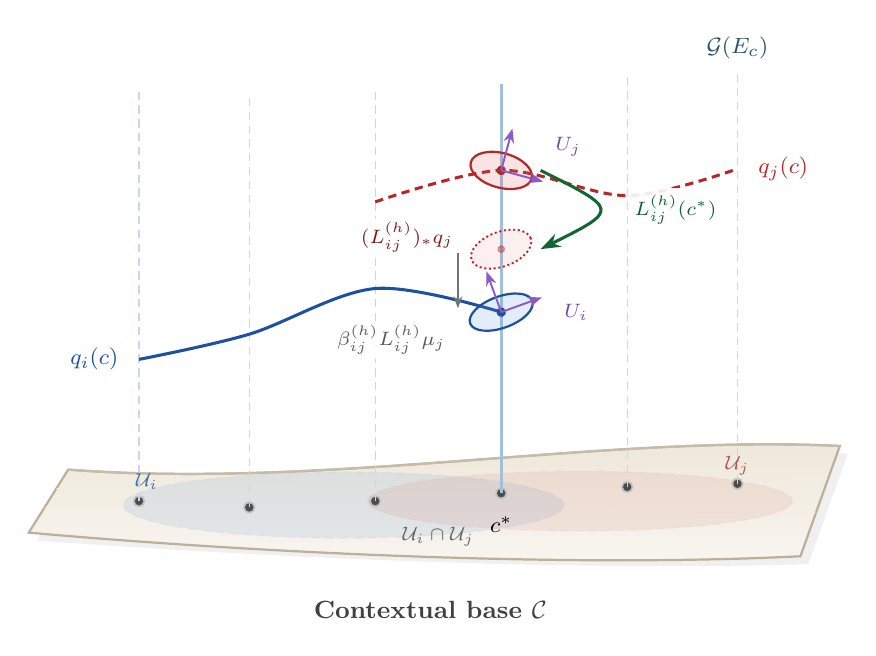
\begin{tikzpicture}[ every node/.style={font=\small}]

\definecolor{fiberblue}{RGB}{70,130,180}
\definecolor{sectionblue}{RGB}{30,80,160}
\definecolor{sectionred}{RGB}{180,40,40}
\definecolor{transportgreen}{RGB}{20,120,60}
\definecolor{gaussblue}{RGB}{100,150,220}
\definecolor{gaussred}{RGB}{220,100,100}
\definecolor{framecol}{RGB}{140,90,200}
\definecolor{basetan}{RGB}{230,220,200}
\definecolor{baseedge}{RGB}{160,140,110}
\definecolor{neighborblue}{RGB}{80,140,210}
\definecolor{neighborred}{RGB}{210,110,100}

\path
  (-0.3,0.1) coordinate (M1)
  (9.5,0.4) coordinate (M2)
  (9.0,-1.0) coordinate (M3)
  (-0.8,-0.7) coordinate (M4);

\filldraw[fill=black!6, draw=none]
  ($(M1)+(0.1,-0.1)$)
  .. controls (3.0,-0.2) and (6.5,0.6) .. ($(M2)+(0.1,-0.1)$)
  -- ($(M3)+(0.1,-0.1)$)
  .. controls (6.0,-1.2) and (2.0,-1.0) .. ($(M4)+(0.1,-0.1)$)
  -- cycle;

\shade[top color=basetan!70, bottom color=basetan!25, draw=baseedge!70, thick]
  (M1)
  .. controls (3.0,-0.15) and (6.5,0.55) .. (M2)
  -- (M3)
  .. controls (6.0,-1.15) and (2.0,-0.95) .. (M4)
  -- cycle;

\draw[baseedge!60, thick]
  (M1) .. controls (3.0,-0.15) and (6.5,0.55) .. (M2);

\foreach \t in {0.3, 0.6} {
  \draw[baseedge!15, very thin]
  ($(M1)!\t!(M4)$) .. controls
  ($($(M1)!\t!(M4)$)!0.4!($(M2)!\t!(M3)$)+(0,0.04)$) and
  ($($(M1)!\t!(M4)$)!0.6!($(M2)!\t!(M3)$)+(-0.02,-0.04)$)
  .. ($(M2)!\t!(M3)$);
}

\node[below, black!75, font=\small\bfseries] at (4.3,-1.45) {Contextual base $\mathcal{C}$};

\coordinate (C1) at (0.6,-0.30);
\coordinate (C2) at (2.0,-0.38);
\coordinate (C3) at (3.6,-0.30);
\coordinate (C4) at (5.2,-0.20);
\coordinate (C5) at (6.8,-0.12);
\coordinate (C6) at (8.2,-0.08);


\filldraw[neighborblue, opacity=0.12, draw=neighborblue!60,
  line width=0.5pt, densely dashed]
  (3.2,-0.35) ellipse (2.8 and 0.42);
\node[neighborblue!80!black, font=\scriptsize] at (0.7,-0.05) {$\mathcal{U}_i$};

\filldraw[neighborred, opacity=0.12, draw=neighborred!60,
  line width=0.5pt, densely dashed]
  (6.2,-0.30) ellipse (2.7 and 0.38);
\node[neighborred!80!black, font=\scriptsize] at (8.2,0.15) {$\mathcal{U}_j$};

\node[black!60, font=\scriptsize] at (4.4,-0.75) {$\mathcal{U}_i \cap \mathcal{U}_j$};

\foreach \c in {C1,C2,C3,C4,C5,C6} {
  \filldraw[black!25] (\c) circle (2pt);
  \filldraw[black!70] (\c) circle (1.3pt);
}

\pgfmathsetmacro{\fh}{5.2}

\foreach \c in {C1,C2,C3,C4,C5,C6} {
  \draw[fiberblue!30, densely dashed, line width=0.4pt]
  (\c) -- ++(0,\fh);
}

\node[above=2pt, fiberblue!60!black, font=\footnotesize]
  at ($(C6)+(0,\fh)$) {$\mathcal{G}(E_c)$};


\coordinate (Si1) at ($(C1)+(0,1.8)$);
\coordinate (Si2) at ($(C2)+(0,2.2)$);
\coordinate (Si3) at ($(C3)+(0,2.7)$);
\coordinate (Si4) at ($(C4)+(0,2.3)$);

\draw[sectionblue, line width=1.1pt]
  plot[smooth, tension=0.55] coordinates {
  (Si1) (Si2) (Si3) (Si4)
  };

\coordinate (Sj3) at ($(C3)+(0,3.8)$);
\coordinate (Sj4) at ($(C4)+(0,4.1)$);
\coordinate (Sj5) at ($(C5)+(0,3.7)$);
\coordinate (Sj6) at ($(C6)+(0,4.0)$);

\draw[sectionred, densely dashed, line width=1.1pt]
  plot[smooth, tension=0.55] coordinates {
  (Sj3) (Sj4) (Sj5) (Sj6)
  };

\node[sectionblue, font=\footnotesize, left=4pt] at (Si1) {$q_i(c)$};
\node[sectionred, font=\footnotesize, right=4pt] at (Sj6) {$q_j(c)$};


\draw[fiberblue!50, line width=1.0pt] (C4) -- ++(0,\fh);

\node[below=5pt, black, font=\footnotesize\itshape] at (C4) {$c^*$};


\begin{scope}[shift={(Si4)}, rotate=20]
  \filldraw[gaussblue, opacity=0.18] (0,0) ellipse (0.42 and 0.20);
  \draw[sectionblue, line width=0.8pt] (0,0) ellipse (0.42 and 0.20);
  \filldraw[sectionblue] (0,0) circle (1.5pt);
\end{scope}

\begin{scope}[shift={(Sj4)}, rotate=-15]
  \filldraw[gaussred, opacity=0.18] (0,0) ellipse (0.40 and 0.22);
  \draw[sectionred, line width=0.8pt] (0,0) ellipse (0.40 and 0.22);
  \filldraw[sectionred] (0,0) circle (1.5pt);
\end{scope}


\begin{scope}[shift={(Si4)}, rotate=20]
  \draw[-{Stealth[length=1.8mm]}, framecol, line width=0.7pt]
  (0,0) -- (0.55,0);
  \draw[-{Stealth[length=1.8mm]}, framecol, line width=0.7pt]
  (0,0) -- (0,0.55);
\end{scope}
\node[framecol!80!black, font=\scriptsize] at ($(Si4)+(0.95,0.0)$) {$U_i$};

\begin{scope}[shift={(Sj4)}, rotate=-15]
  \draw[-{Stealth[length=1.8mm]}, framecol, line width=0.7pt]
  (0,0) -- (0.55,0);
  \draw[-{Stealth[length=1.8mm]}, framecol, line width=0.7pt]
  (0,0) -- (0,0.55);
\end{scope}
\node[framecol!80!black, font=\scriptsize] at ($(Sj4)+(0.85,0.30)$) {$U_j$};


\coordinate (Ghost) at ($(Si4)+(0,0.8)$);
\begin{scope}[shift={(Ghost)}, rotate=20]
  \filldraw[gaussred, opacity=0.10] (0,0) ellipse (0.40 and 0.22);
  \draw[sectionred, densely dotted, line width=0.7pt] (0,0) ellipse (0.40 and 0.22);
  \filldraw[sectionred, opacity=0.4] (0,0) circle (1.2pt);
\end{scope}

\node[sectionred!70!black, font=\scriptsize,
  fill=white, fill opacity=0.9, text opacity=1,
  inner sep=1.5pt, rounded corners=1pt, anchor=east]
  (pushforwardlabel) at ($(Ghost)+(-0.55,0.15)$) {$(L_{ij}^{(h)})_*q_j$};

\draw[-{Stealth[length=2.5mm, width=1.8mm]},
  transportgreen!85!black, line width=1.1pt]
  ($(Sj4)+(0.5,0)$)
  .. controls ($(Sj4)+(1.5,-0.5)$) and ($(Ghost)+(1.5,0.5)$)
  .. ($(Ghost)+(0.5,0)$);

\node[transportgreen!80!black, font=\scriptsize\bfseries,
  fill=white, fill opacity=0.9, text opacity=1,
  inner sep=2.5pt, rounded corners=2pt, anchor=west]
  at ($(Sj4)!0.5!(Ghost)+(1.6,0)$) {$L_{ij}^{(h)}(c^*)$};


\draw[-{Stealth[length=1.5mm]},
  black!55, line width=0.6pt]
  ($(Ghost)+(-0.55,-0.05)$) -- ($(Si4)+(-0.55,0.05)$);

\node[black!65, font=\scriptsize,
  fill=white, fill opacity=0.9, text opacity=1,
  inner sep=1.5pt, rounded corners=1pt, anchor=east]
  (messagelabel) at ($(Si4)+(-0.65,-0.35)$) {$\beta_{ij}^{(h)}L_{ij}^{(h)}\mu_j$};

\end{tikzpicture}
}
\caption{\textbf{Local Gaussian sections and directed communication links.}
The curved surface represents the contextual base of the principal bundle; the curves are sections of its associated Gaussian-state bundle over overlapping neighborhoods. At a shared context \(c^*\), the local frames accompany the state glyphs. For one communication head indexed by \(h\), the green arrow applies \(L_{ij}^{(h)}=U_iO_hT_hU_j^{-1}\) to the sender. The dotted contour depicts its Gaussian pushforward; the gray arrow identifies the weighted mean contribution to the receiver. A full-rank link is illustrated; a lower-rank link may produce a singular pushforward. The receiver's state need not equal that pushforward. Routing uses the separate comparison channel in Figure~\ref{fig:comparison_content_interfaces}. The finite token construction requires no smooth contextual base.}
\label{fig:link_construction}
\end{figure}

\subsection{Principal bundle and associated Gaussian states}
\label{sec:principal_construction}

The geometric construction begins with a principal bundle of reference frames over a space of contexts. Let \(\mathcal C\) be a smooth contextual base and take \(G=\mathrm{GL}(K,\mathbb R)\). A principal bundle
\begin{equation}
\pi:\mathcal P\longrightarrow\mathcal C
\label{eq:principal_bundle}
\end{equation}
carries a free right action \(n\mapsto n\cdot g\) that preserves \(\pi\) and is transitive on each fiber. Locally, \(\mathcal P|_{\mathcal U}\simeq\mathcal U\times G\), with the group acting on the second factor. Thus a principal fiber consists of frame choices; choosing one frame identifies the fiber with \(G\). The probabilistic states are attached to this principal structure through associated bundles \citep{nakahara2003geometry,frankel2011geometry}.

Let \(\mathsf V=\mathbb R^K\) carry the defining representation of \(G\), and let
\begin{equation}
\mathcal B=\{\mathcal N(\mu,\Sigma):\mu\in\mathsf V,\ \Sigma\succ0\},
\qquad
\rho(g)\mathcal N(\mu,\Sigma)=\mathcal N(g\mu,g\Sigma g^\top).
\label{eq:gaussian_associated_action}
\end{equation}
The vector and Gaussian statistical bundles are
\begin{equation}
E=\mathcal P\times_G\mathsf V,
\qquad
\mathcal G(E)=\mathcal P\times_\rho\mathcal B.
\label{eq:associated_state_bundles}
\end{equation}
For the statistical bundle, the quotient convention is
\begin{equation}
(n\cdot g,b)\sim(n,\rho(g)b).
\label{eq:associated_quotient}
\end{equation}
Equivalently, \((n,b)\) and \((n\cdot g,\rho(g^{-1})b)\) represent the same associated point. The analogous relation uses \(v\mapsto gv\) for the vector bundle. The principal bundle carries gauge freedom, the vector bundle carries latent values, and the associated statistical bundle carries distributions over those values.

An agent over a contextual region \(\mathcal U_i\) selects a local principal section \(u_i\) and maintains belief and prior sections:
\begin{equation}
\begin{aligned}
u_i&:\mathcal U_i\longrightarrow\mathcal P,
&\pi\circ u_i&=\operatorname{id}_{\mathcal U_i},\\
q_i,p_i&\in\Gamma\bigl(\mathcal G(E)|_{\mathcal U_i}\bigr).
\end{aligned}
\label{eq:agent_bundle_sections}
\end{equation}
Here \(\Gamma\) denotes smooth sections, and the belief and prior have coordinates \((\mu_i,\Sigma_i)\) and \((\mu_{p,i},\Sigma_{p,i})\) in the section \(u_i\). Communication additionally uses one reference trivialization \(\sigma_0\) of \(\mathcal P\) on its working domain. The frame field is the relative element \(U_i\) defined by \(u_i=\sigma_0\cdot U_i^{-1}\), so that \(\xi_i=U_i^{-1}\mu_i\) are the \(\sigma_0\)-coordinates of the same vector. Identifying the fiber with its coordinates in the section \(u_i\), written \(E_c\), the frame is the linear isomorphism \(U_i(c):\mathsf V\to E_c\) that converts \(\sigma_0\)-coordinates into \(u_i\)-coordinates. On overlaps, agents can maintain different Gaussian sections at the same context. They are not required to be local representatives of one common belief. Figure~\ref{fig:link_construction} illustrates these associated statistical sections and their local frames. The attention construction uses this belief/prior sector; it does not require an additional bundle of generative-model parameters.

For token attention, the contextual dependence is evaluated at a fixed context \(c_0\), while \(i\in\mathcal I=\{0,\ldots,N-1\}\) labels the token agents. Keeping a separately labeled copy of the fiber for each token is the pullback along the constant map \(\iota:\mathcal I\to\mathcal C\), \(\iota(i)=c_0\):
\begin{equation}
\mathcal P_{\mathcal I}=\iota^*\mathcal P,
\qquad E_{\mathcal I}=\iota^*E.
\label{eq:token_bundle_pullback}
\end{equation}
Write \(E_i\) for the vector fiber at token \(i\). This notation distinguishes token incidence from the contextual base of the general construction. Because \(\iota\) is constant, \(\iota^*\mathcal P=\mathcal I\times\mathcal P_{c_0}\) canonically. The token construction therefore sees no connection, curvature, or topology of \(\mathcal P\), and its gauge group is \(G^N\), on which the contextual gauge group acts only through the diagonal. Placing tokens at distinct contexts \(\iota(i)=c_i\) and realizing links by parallel transport along declared base curves would make the contextual connection enter the attention operator. The section of each token agent and the reference trivialization give \(U_i:\mathsf V\to E_i\), and its statistical fiber is
\begin{equation}
\mathcal G(E_i)=\{\mathcal N(\mu,\Sigma):\mu\in E_i,\ \Sigma\succ0\}.
\label{eq:overview_statistical_fiber}
\end{equation}
The state and its local prior, expressed in the same local coordinates, are
\begin{align}
q_i&=\mathcal N(\mu_i,\Sigma_i),\qquad \Sigma_i\succ0,\label{eq:gaussian_states}\\
p_i&=\mathcal N(\mu_{p,i},\Sigma_{p,i}),\qquad \Sigma_{p,i}\succ0.\label{eq:base_priors}
\end{align}
Their reference-coordinate representation, in \(\sigma_0\)-coordinates, is obtained through the frame:
\begin{equation}
\widetilde q_i=(U_i^{-1})_*q_i
=\mathcal N(\xi_i,C_i),\qquad
\xi_i=U_i^{-1}\mu_i,\quad
C_i=U_i^{-1}\Sigma_iU_i^{-\top}.
\label{eq:overview_reference_state}
\end{equation}
The covariance is an unrestricted positive-definite matrix. The frame determines this coordinate identification; the additional communication interfaces determine which directions another agent receives.

A general contextual principal bundle need not admit a global section. The factorized attention formulas use the reference trivialization \(\sigma_0\) on their working domain; on the finite token pullback this trivialization is canonical. The communication graph is additional data; the matrix links on it are determined by the frames, the shared interfaces, and the routing weights. A link \(L_{ij}:E_j\to E_i\) can be singular, so it is not in general a principal-bundle transition function or a group-valued parallel transport. Sections~\ref{sec:role_measurements}--\ref{sec:matrix_link_fields} construct these links from comparison and content interfaces while retaining the underlying principal-bundle structure.

\subsection{Coordinate independence}
\label{sec:glk_invariance}

By Eq.~\eqref{eq:associated_quotient}, a rechoice \(u_i\mapsto u_i\cdot g_i^{-1}\) of the section of agent \(i\), with \(\sigma_0\) held fixed, changes the coordinates as in Eq.~\eqref{eq:passive_site_action} below. These rechoices are independent passive coordinate changes at the token sites. A change of \(\sigma_0\) is the common reference-basis change \(U_i\mapsto U_ia\) of Section~\ref{sec:role_measurements}. Under such a passive site change, the same construction is represented by
\begin{equation}
(\mu_i,\Sigma_i,U_i)\mapsto
(g_i\mu_i,g_i\Sigma_i g_i^\top,g_iU_i),
\qquad g_i\in\mathrm{GL}(K).
\label{eq:passive_site_action}
\end{equation}
The reference moments \((\xi_i,C_i)\) are unchanged. Reference-space interface parameters are held fixed under this passive action; covectors transform contragrediently. The link endpoint law will follow by composing the sending and receiving maps in Section~\ref{sec:matrix_link_fields}.

The standard change-of-variables identity underlying this distinction is
\begin{equation}
D_{\mathrm{KL}}(A_*P\|A_*Q)=D_{\mathrm{KL}}(P\|Q),
\qquad A\in\mathrm{GL}(K).
\label{eq:glk_invariance}
\end{equation}
Both densities acquire the same Jacobian factor, which cancels in their ratio \citep{Amari2016}. The same argument applies to \(f\)-divergences, and the data-processing inequality applied to \(A\) and \(A^{-1}\) gives equality for every R\'enyi order \citep[Thm.~9]{vanErvenHarremoes2014}. This common invertible change of coordinates is distinct from a rank-reducing measurement or a change to the learned interfaces.

A useful frame parametrization is \(U_i=\exp(X_{x_i})\exp(Y_i)\), combining token and positional factors. Its determinants are positive. The passive law above is defined for arbitrary invertible frames; a single real exponential is not a global chart of \(\mathrm{GL}^+(K)\), and a product of real exponentials need not have a real logarithm \citep{culver1966existence}. These chart restrictions do not alter the link's endpoint law.

The subsequent covariance statements concern the attention operator with its full Gaussian data transformed consistently. Section~\ref{sec:passive_covariance} states what that covariance does and does not constrain and where the frames act in the rest of the predictor, and Supplementary Section~\ref{sec:nonlinear_gaussian_scope} gives explicit limits on identifying its nonlinear operations with full Gaussian propagation.

\subsection{Communication layers, heads, and comparison spaces}
\label{sec:role_measurements}

A layer is one communication update applied to the collection of token states. The index \(\ell\) counts successive updates: \(q_i^{(\ell)}=\mathcal N(\mu_i^{(\ell)},\Sigma_i^{(\ell)})\) is the state entering layer \(\ell\), and \(q_i^{(\ell+1)}\) is its output. The reference moments \(\xi_i^{(\ell)},C_i^{(\ell)}\) are defined by Eq.~\eqref{eq:overview_reference_state} for that input state.

Each layer contains \(H\) communication heads, indexed by \(h=1,\ldots,H\). A head is one channel with its own source comparison and content maps; its weighted messages are combined with those of the other heads. This definition does not require the heads to partition the state or coincide with irreducible frame blocks. For each head choose two real vector spaces,
\begin{equation}
H_h^{\mathrm{cmp}}=\mathbb R^{r_h},
\qquad
H_h^{\mathrm{val}}=\mathbb R^{s_h}.
\label{eq:head_channel_spaces}
\end{equation}
The superscript \(\mathrm{cmp}\) denotes the comparison space, in which source compatibility is measured; \(\mathrm{val}\) denotes the content or value space, through which the transmitted message passes. The positive integers \(r_h\) and \(s_h\) are their dimensions. These spaces are shared across token positions and need not have the same dimension.

The layer's interfaces have the declared types
\begin{align}
S_{Q,h}^{(\ell)},S_{K,h}^{(\ell)}
&:\mathsf V\longrightarrow H_h^{\mathrm{cmp}},\\
T_h^{(\ell)}&:\mathsf V\longrightarrow H_h^{\mathrm{val}},
\qquad
O_h^{(\ell)}:H_h^{\mathrm{val}}\longrightarrow\mathsf V.
\label{eq:head_interface_types}
\end{align}
The query map \(S_Q\) measures the receiver and the key map \(S_K\) measures a candidate sender; both have full row rank, hence \(r_h\le K\). The value map \(T\) extracts content, and the output map \(O\) places it in reference state coordinates. Their composition with local frames is developed in Section~\ref{sec:matrix_link_fields}. Superscripts \((\ell,h)\) identify a layer and head, and layer indices are suppressed when one layer is fixed. Matrices act on column vectors, and \(ij\) denotes a map from sender \(j\) to receiver \(i\).

The maps are specified in the chosen reference basis. Under a common reference-basis change \(U_i\mapsto U_i a\), their representations change as \(S_Q\mapsto S_Qa\), \(S_K\mapsto S_Ka\), \(T\mapsto Ta\), and \(O\mapsto a^{-1}O\), while \(\xi_i\mapsto a^{-1}\xi_i\) and \(C_i\mapsto a^{-1}C_i a^{-\top}\). Thus the measured laws and the content link are unchanged. Holding the interface matrices fixed while making this reference-basis change would specify a different communication rule.

The query and key Gaussian pushforwards therefore occupy the same comparison space:
\begin{align}
q_{Q,i}^{(\ell,h)}
&=\mathcal N\bigl(S_{Q,h}^{(\ell)}\xi_i^{(\ell)},
 S_{Q,h}^{(\ell)}C_i^{(\ell)}S_{Q,h}^{(\ell)\top}\bigr),\label{eq:relational_query_law}\\
p_{K,j}^{(\ell,h)}
&=\mathcal N\bigl(S_{K,h}^{(\ell)}\xi_j^{(\ell)},
 S_{K,h}^{(\ell)}C_j^{(\ell)}S_{K,h}^{(\ell)\top}\bigr),\label{eq:relational_key_law}\\
D_{ij}^{(\ell,h)}
&=D_{\mathrm{KL}}\bigl(q_{Q,i}^{(\ell,h)}\|p_{K,j}^{(\ell,h)}\bigr).
\label{eq:relational_role_kl}
\end{align}
Because $C_i^{(\ell)}\succ0$ and each comparison map has full row rank, the reduced covariance is positive definite: for $y\ne0$, $y^\top SCS^\top y=(S^\top y)^\top C(S^\top y)>0$. These are full reduced covariances, including their off-diagonal entries. Thus the construction uses nonsingular distributions in the measured space, rather than treating a singular ambient projection as a $K$-dimensional Gaussian density.

When $S_Q=S_K=S$, the score compares a common measurement of the two reference beliefs. When $S_Q\ne S_K$, it compares distinct role observables identified in one comparison space. The latter is an additional modeling choice. The maps are learned interface parameters and are generally rectangular; they are not individually invertible gauge transformations. Full input scope means that every head's maps read all $K$ coordinates, as learned projections do in conventional multi-head attention \citep{vaswani2017attention}. It does not mean that the comparison dimension equals $K$.

The routing costs also do not depend on a basis of the comparison space. Equation~\eqref{eq:glk_invariance} applied in \(H_h^{\mathrm{cmp}}\) shows that \((S_{Q,h},S_{K,h})\mapsto(AS_{Q,h},AS_{K,h})\), \(A\in\mathrm{GL}(r_h)\), leaves every \(D_{ij}^{(\ell,h)}\) unchanged, and tied maps enter only through their row space. This cogredient redundancy differs from the contragredient redundancy \((W_Q,W_K)\mapsto(W_QA,W_KA^{-\top})\) of dot-product scores; the two share only \(A\in\mathrm O(r_h)\), the residual freedom of whitening in Proposition~\ref{prop:projected_dot_product}. In particular, a common rescaling of \(S_{Q,h}\) and \(S_{K,h}\) does not change the routing temperature. The content maps carry the analogous redundancy \((T_h,O_h)\mapsto(BT_h,O_hB^{-1})\), \(B\in\mathrm{GL}(s_h)\). Only \(H_h^{\mathrm{cmp}}\) and \(H_h^{\mathrm{val}}\) as abstract vector spaces are determined by the model; their bases are internal parameter redundancies. Gradient flow on a loss that depends on these maps only through the costs and messages therefore conserves \(S_{Q,h}S_{Q,h}^\top+S_{K,h}S_{K,h}^\top\) and \(T_hT_h^\top-O_h^\top O_h\) \citep{du2018balanced,Kunin2021NeuralMechanics}, whereas adaptive optimizers without weight decay can drift along these directions.


\subsection{Matrix links, projections, and frame transport}
\label{sec:matrix_link_fields}

Communication uses selected directions of an agent's framed state. The mathematical meaning of using a subset of a frame is that a receiving or sending map accesses a lower-dimensional observable of the state expressed in that frame. These maps also set gains and identify transmitted directions with received directions. They need not select coordinate entries, define orthogonal projections, or select a subset of group elements. The possible analogy with information coding is an interpretation to develop; no coding theorem or channel-capacity claim is assumed here.

Fix a layer and suppress its index. The content interfaces \(T_h,O_h\) of Eq.~\eqref{eq:head_interface_types} compose with the local frames to determine a directed map from the sender's state space to the receiver's. Write \(A_{Q,i,h}=S_{Q,h}U_i^{-1}\) and \(A_{K,i,h}=S_{K,h}U_i^{-1}\) for the local comparison measurements, \(\mathsf S_{j,h}=T_hU_j^{-1}\) and \(\mathsf R_{i,h}=U_iO_h\) for the content endpoints, and \(G_i=U_i^{-\top}U_i^{-1}\) for the local metric induced by the Euclidean reference inner product. Table~\ref{tab:link_conventions} collects the geometric data and conventions, and Figure~\ref{fig:comparison_content_interfaces} shows the comparison and content interfaces of one head.

\begin{table}[t]
\centering
\small
\renewcommand{\arraystretch}{1.12}
\begin{tabularx}{\textwidth}{@{}lX@{}}
\toprule
Object & Meaning, domain, and role \\
\midrule
$N,K,H,B$ & Number of positions, state dimension, communication heads, and frame blocks \\
$q_i,p_i$ & Full Gaussian state and local prior on $E_i$ \\
$\xi_i,C_i$ & Reference moments $U_i^{-1}\mu_i$ and $U_i^{-1}\Sigma_iU_i^{-\top}$ \\
$\pi_{ij},\beta_{ij},\tau_h$ & Source prior, routing probability, and positive headwise temperature \\

$U_i$, $G_i=U_i^{-\top}U_i^{-1}$ & Frame $\mathsf V\to E_i$ and local metric induced by the Euclidean reference metric \\
$S_{Q,h},S_{K,h}$ & Full-row-rank maps $\mathsf V\to H_h^{\mathrm{cmp}}=\mathbb R^{r_h}$ defining comparison observables \\
$T_h,O_h$ & Sending map $\mathsf V\to H_h^{\mathrm{val}}=\mathbb R^{s_h}$ and receiving map $H_h^{\mathrm{val}}\to\mathsf V$ \\
$A_{Q,i,h},A_{K,i,h}$ & Local measurements $S_{Q,h}U_i^{-1},S_{K,h}U_i^{-1}:E_i\to H_h^{\mathrm{cmp}}$ \\
$\mathsf S_{j,h},\mathsf R_{i,h}$ & Content endpoints $T_hU_j^{-1}:E_j\to H_h^{\mathrm{val}}$ and $U_iO_h:H_h^{\mathrm{val}}\to E_i$ \\
$L_{ij}^{(h)}$, $\mathcal M_{ij}$ & Content link $\mathsf R_{i,h}\mathsf S_{j,h}$ and routed sum in $\operatorname{Hom}(E_j,E_i)$ \\
$\Omega_{ij}$, $\Theta_{ij}$ & Flat reference identification $U_iU_j^{-1}$ and, only when separately specified, invertible connection transport \\
\bottomrule
\end{tabularx}
\caption{Types and conventions for projection-induced links. Comparison and content spaces are distinct even when their dimensions agree. Layer indices are suppressed.}
\label{tab:link_conventions}
\end{table}

\subsubsection{Content links and selective communication}

The content factors define an ambient matrix link without requiring either factor to be square:
\begin{equation}
L_{ij}^{(h)}=\mathsf R_{i,h}\mathsf S_{j,h}
=U_iO_hT_hU_j^{-1}:E_j\longrightarrow E_i.
\label{eq:main_content_link}
\end{equation}
Under $U_i'=g_iU_i$ and $(\mu_i',\Sigma_i')=(g_i\mu_i,g_i\Sigma_i g_i^\top)$, direct substitution gives
\begin{equation}
\mathsf S_{j,h}'=\mathsf S_{j,h}g_j^{-1},\qquad
\mathsf R_{i,h}'=g_i\mathsf R_{i,h},\qquad
L_{ij}^{(h)\prime}=g_iL_{ij}^{(h)}g_j^{-1}.
\label{eq:main_link_endpoint_law}
\end{equation}
This is an endpoint covariance law for the complete geometric data. It does not say that a fixed rectangular matrix commutes with every $g_i$.

The receiving image is $U_i\operatorname{im}O_h$; the invisible sending directions are $\ker(T_hU_j^{-1})$. With the metric $G_j$ in Table~\ref{tab:link_conventions}, the orthogonal complement of that kernel is $U_j\operatorname{im}T_h^\top$. Indeed, $\langle U_jx,U_jy\rangle_{G_j}=x^\top y$, reducing this statement to the Euclidean identity $(\ker T_h)^\perp=\operatorname{im}T_h^\top$. The Fisher metric of the Gaussian location family, $\Sigma_j^{-1}=U_j^{-\top}C_j^{-1}U_j^{-1}$, transforms in the same way without a reference inner product; in that metric the complement is $U_jC_j\operatorname{im}T_h^\top$, and the Gaussian lift of Eq.~\eqref{eq:comparison_gaussian_lift} below is the minimal-norm right inverse of the query map. Sending, receiving, and comparison subspaces may overlap. Their dimensions do not impose a partition of the frame, and $O_hT_h$ is generally neither orthogonal nor idempotent.

For invariant scalar routing weights, define
\begin{align}
\mathcal M_{ij}&=\sum_h\beta_{ij}^{(h)}L_{ij}^{(h)}
=U_i\left(\sum_h\beta_{ij}^{(h)}O_hT_h\right)U_j^{-1},\\
m_i&=\sum_j\mathcal M_{ij}\mu_j.
\label{eq:main_routed_link}
\end{align}
Equation~\eqref{eq:main_link_endpoint_law} gives $\mathcal M_{ij}'=g_i\mathcal M_{ij}g_j^{-1}$ and $m_i'=g_im_i$. The projected Gaussian routing below supplies the required scalar invariance: $\xi_i'=\xi_i$ and $C_i'=C_i$, so all comparison laws and their divergences are unchanged. The attention residual $\mu_i+m_i$ consequently has the same vector covariance.

Each head has rank at most $s_h$, but the total link obeys only
\begin{equation}
\operatorname{rank}\mathcal M_{ij}
\le\min\left(K,\sum_hs_h\right).
\label{eq:main_link_rank}
\end{equation}
For example, at $K=2$, take $O_1T_1=\operatorname{diag}(1,0)$ and $O_2T_2=\operatorname{diag}(0,1)$. Positive weights produce the invertible reference operator $\operatorname{diag}(\beta_{ij}^{(1)},\beta_{ij}^{(2)})$. Conversely, a single head with $s_h<K$ cannot be a $\mathrm{GL}(K)$ element. The realized matrices also remain in the span of the shared $O_hT_h$ at a fixed layer; they are not unrestricted independent edge parameters.

\begin{figure}[htbp]
\centering
\resizebox{0.98\textwidth}{!}{%
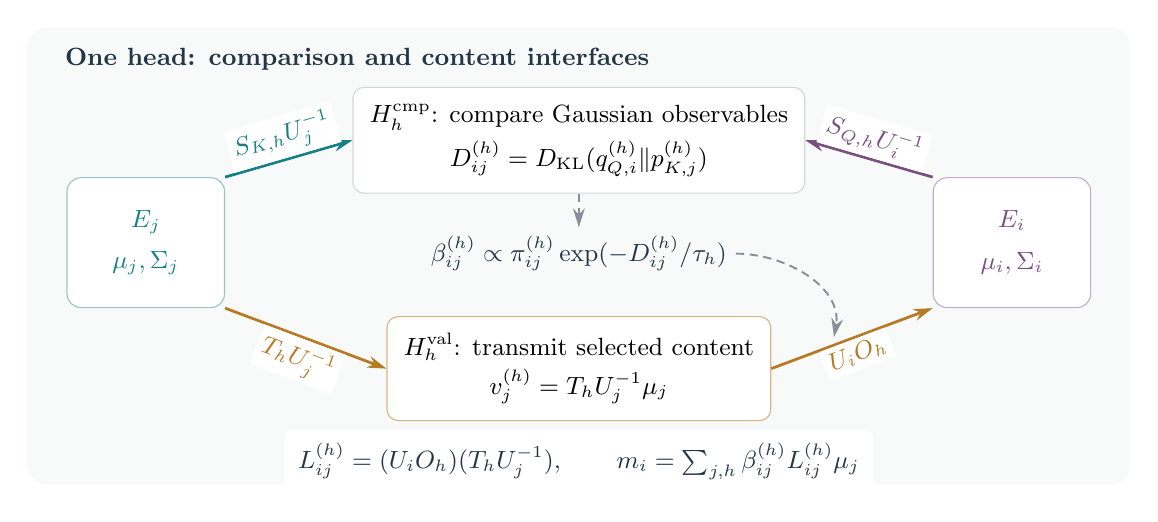
\begin{tikzpicture}[
  >={Stealth[length=2.4mm,width=1.5mm]},
  every node/.style={font=\small},
  paneltitle/.style={font=\small\bfseries,text=ink,anchor=west},
  port/.style={rounded corners=5pt,draw=ink!20,fill=white,minimum width=2.0cm,minimum height=1.65cm,align=center,inner sep=8pt},
  channel/.style={rounded corners=4pt,draw=ink!20,fill=white,minimum width=4.3cm,minimum height=1.0cm,align=center,inner sep=6pt},
  map/.style={->,line width=1.0pt},
  maplabel/.style={font=\small,fill=white,inner sep=2pt},
  control/.style={->,densely dashed,draw=ink!55,line width=.7pt}
]
\definecolor{ink}{HTML}{243545}
\definecolor{sender}{HTML}{167F86}
\definecolor{receiver}{HTML}{775080}
\definecolor{linkgold}{HTML}{B67A23}
\definecolor{paperblue}{HTML}{F1F6F8}

\fill[ink!3,rounded corners=7pt] (0,-.72) rectangle (14,5.08);
\node[paneltitle] at (.35,4.68) {One head: comparison and content interfaces};

\node[port,draw=sender!45,text=sender] (source) at (1.50,2.35)
  {\(E_j\)\\[4pt]\(\mu_j,\Sigma_j\)};
\node[port,draw=receiver!45,text=receiver] (target) at (12.50,2.35)
  {\(E_i\)\\[4pt]\(\mu_i,\Sigma_i\)};
\node[channel] (cmp) at (7.0,3.65)
  {\(H_h^{\mathrm{cmp}}\): compare Gaussian observables\\[3pt]
   \(D_{ij}^{(h)}=D_{\mathrm{KL}}(q_{Q,i}^{(h)}\|p_{K,j}^{(h)})\)};
\node[channel,draw=linkgold!55] (val) at (7.0,.75)
  {\(H_h^{\mathrm{val}}\): transmit selected content\\[3pt]
   \(v_j^{(h)}=T_hU_j^{-1}\mu_j\)};

\draw[map,sender] (source.north east) -- node[maplabel,above,sloped] {\(S_{K,h}U_j^{-1}\)} (cmp.west);
\draw[map,receiver] (target.north west) -- node[maplabel,above,sloped] {\(S_{Q,h}U_i^{-1}\)} (cmp.east);
\draw[map,linkgold] (source.south east) -- node[maplabel,below,sloped] {\(T_hU_j^{-1}\)} (val.west);
\draw[map,linkgold] (val.east) -- node[maplabel,below,sloped] {\(U_iO_h\)} (target.south west);
\node[font=\small,text=ink,fill=ink!3,inner sep=3pt] (route) at (7.0,2.21)
  {\(\beta_{ij}^{(h)}\propto\pi_{ij}^{(h)}\exp(-D_{ij}^{(h)}/\tau_h)\)};
\draw[control] (cmp.south) -- (route.north);
\draw[control] (route.east) to[out=0,in=80] (10.24,1.15);
\node[font=\small,text=ink,fill=white,rounded corners=3pt,inner sep=5pt] at (7.0,-.43)
  {\(L_{ij}^{(h)}=(U_iO_h)(T_hU_j^{-1}),\qquad
     m_i=\sum_{j,h}\beta_{ij}^{(h)}L_{ij}^{(h)}\mu_j\)};
\end{tikzpicture}
}
\caption{\textbf{Separate comparison and content interfaces.}
Query and key maps send Gaussian observables into a common comparison space, where their divergence determines the routing weight. The content maps \(T_hU_j^{-1}\) and \(U_iO_h\) extract and place the transmitted mean. Their composition is the matrix link \(L_{ij}^{(h)}\); dashed arrows show scalar routing control, not an additional state map. The Gibbs weights are derived in Section~\ref{sec:mixture_derivation}.}
\label{fig:comparison_content_interfaces}
\end{figure}

\subsubsection{Comparison maps and induced links}

The query and key maps first define the comparison cospan
\begin{equation}
E_i\xrightarrow{A_{Q,i,h}}H_h^{\mathrm{cmp}}
\xleftarrow{A_{K,j,h}}E_j.
\label{eq:comparison_cospan}
\end{equation}
The Gaussian observables of Eqs.~\eqref{eq:relational_query_law} and~\eqref{eq:relational_key_law} occupy this common comparison space. A cospan compares two observables; it does not by itself choose a map back from the comparison space to $E_i$.

The distinction can be seen directly in the mean cross term of the Gaussian KL. Suppress $h$, and put $P_{K,j}=(A_{K,j}\Sigma_jA_{K,j}^\top)^{-1}$. The comparison tensor is
\begin{equation}
B_{ij}=A_{Q,i}^\top P_{K,j}A_{K,j},\qquad
B_{ij}'=g_i^{-\top}B_{ij}g_j^{-1}.
\label{eq:comparison_bilinear_tensor}
\end{equation}
It maps $E_j$ to $E_i^*$, with invariant scalar $\mu_i^\top B_{ij}\mu_j$. A vector link instead maps $E_j$ to $E_i$. A declared receiver metric can raise the first index: $G_i^{-1}B_{ij}$ then obeys the link law because $G_i'=g_i^{-\top}G_ig_i^{-1}$. The covariance $\Sigma_i$, viewed as a map $E_i^*\to E_i$, supplies another such choice; with the Fisher metric $G_i=\Sigma_i^{-1}$ the two choices coincide. Neither choice is an inverse of the rectangular query map.

A more specific lift uses the receiver's Gaussian geometry. Define
\begin{align}
R_{Q,i}&=C_iS_Q^\top(S_QC_iS_Q^\top)^{-1},\qquad S_QR_{Q,i}=I_{r_h},\\
L_{ij}^{\mathrm{cmp}}
&=U_iR_{Q,i}S_KU_j^{-1}.
\label{eq:comparison_gaussian_lift}
\end{align}
For every $y\in\mathbb R^{r_h}$, $R_{Q,i}y$ is the unique minimizer of $\delta^\top C_i^{-1}\delta$ subject to $S_Q\delta=y$. To check this, write $\delta=R_{Q,i}y+w$ with $S_Qw=0$. Then $(R_{Q,i}y)^\top C_i^{-1}w=y^\top(S_QC_iS_Q^\top)^{-1}S_Qw=0$, so the objective is its value at $R_{Q,i}y$ plus $w^\top C_i^{-1}w$. This also identifies the lift in the Gaussian conditional mean,
\begin{equation}
\mathbb E[X_i\mid S_QX_i=y]
=\xi_i+R_{Q,i}(y-S_Q\xi_i),
\quad X_i\sim\mathcal N(\xi_i,C_i).
\label{eq:comparison_conditional_mean}
\end{equation}
For the conditional identity, the Gaussian residual $X_i-\xi_i-R_{Q,i}(S_QX_i-S_Q\xi_i)$ has zero cross covariance with $S_QX_i$, since $C_iS_Q^\top-R_{Q,i}S_QC_iS_Q^\top=0$. Its joint Gaussian characteristic function therefore factors, making the residual independent of the measurement and giving Eq.~\eqref{eq:comparison_conditional_mean}. Thus $L_{ij}^{\mathrm{cmp}}$ is a precise state-dependent comparison link induced by a specified lift. Its covariance follows because $R_{Q,i}$ is unchanged by the passive site action. It transports a comparison displacement into the receiver; the complete conditional mean includes the affine centering term in Eq.~\eqref{eq:comparison_conditional_mean}. This construction gives $S_Q$ and $S_K$ a precise induced-link interpretation. It is distinct from the independently chosen content link $L_{ij}^{(h)}$ built from $T_h,O_h$; equality would require additional conditions on those maps.

\subsubsection{Composition and the flat reference specialization}
\label{sec:flat_identification}

Let $M_h=O_hT_h$. For an unweighted head, intermediate frame factors cancel:
\begin{align}
L_{ij}^{(h)}L_{jk}^{(h)}-L_{ik}^{(h)}
&=U_iO_h(T_hO_h-I_{s_h})T_hU_k^{-1},\\
L_{i_0i_1}^{(h)}\cdots L_{i_{a-1}i_a}^{(h)}
&=U_{i_0}M_h^aU_{i_a}^{-1}.
\label{eq:main_link_composition}
\end{align}
The defect measures repeated receiving-to-sending processing. If $T_hO_h=I_{s_h}$, then $L_{ij}^{(h)}$ identifies $U_j\operatorname{im}O_h$ with $U_i\operatorname{im}O_h$ and composes flatly on these subspaces; its ambient self-map is a projector. At $K=s_h=1$, $U_i=1$, $T_h=1$, and $O_h=2$, the one-edge map is $2$ while the two-edge map is $4$. Even invertibility therefore does not make the shared processing family a flat reference transport. Paths of the same length and endpoints still agree for this unweighted, shared-head specialization. Routed mixtures can depend on the intermediate sites through their coefficients. Conversely, if \(O_h\) has full column rank and \(T_h\) has full row rank, a vanishing composition defect implies \(T_hO_h=I_{s_h}\): multiply the defect by a left inverse of \(O_h\) and a right inverse of \(T_h\). Without these rank assumptions the converse can fail.

The separate reference identification is
\begin{equation}
\Omega_{ij}=U_iU_j^{-1},\qquad
k_j\mapsto\Omega_{ij}k_j.
\label{eq:gauge_frame_rotation}
\end{equation}
It is recovered from a content link when $O_hT_h=I_K$. When the frames are each represented by one exponential, it equals $e^{\phi_i}e^{-\phi_j}$; the chart restrictions discussed above remain applicable.
\begin{remark}[Flat reference identification]
\label{rem:flat_identification}
For any invertible frames and any finite sequence of sites, successive factors cancel, $\Omega_{ij}\Omega_{jk}=U_iU_k^{-1}=\Omega_{ik}$. The ordered product of the $\Omega$ maps therefore depends only on its endpoints, and every closed product equals $I_K$; in particular $\Omega_{ij}\Omega_{jk}\Omega_{ki}=I_K$. The reference identification is pure gauge: it is the coboundary of the frame field.
\end{remark}
The global reference space supplies this trivialization explicitly. A finite discrete base has no overlap or continuum topology obstruction here; the graph may nevertheless support independent connection data with nonidentity cycle products. The identity just proved applies to $\Omega$, not to every matrix communication link.

For a declared closed walk \(\gamma=(i_0,\ldots,i_r=i_0)\) and endpoint-covariant edge matrices \(L_{ij}:E_j\to E_i\), define
\begin{align}
\mathcal H_\gamma(L)&=L_{i_0i_1}\cdots L_{i_{r-1}i_0},\\
\mathcal H_\gamma(L)'&=g_{i_0}\mathcal H_\gamma(L)g_{i_0}^{-1},\\
\mathcal W_\gamma(L)&=\operatorname{Tr}\mathcal H_\gamma(L).
\label{eq:main_matrix_loop_trace}
\end{align}
Intermediate gauge factors cancel, and cyclicity of trace proves that \(\mathcal W_\gamma\) is invariant even for singular links. It is not a complete invariant of the loop matrix. For routed links, write \(M_{ij}=\sum_h\beta_{ij}^{(h)}M_h\). Then
\begin{equation}
\mathcal H_\gamma(\mathcal M)
=U_{i_0}\bigl(M_{i_0i_1}\cdots M_{i_{r-1}i_0}\bigr)U_{i_0}^{-1}.
\label{eq:main_routed_loop_body}
\end{equation}
Expanding the product, each routed loop trace is a polynomial in the routing weights with loop-independent coefficients \(\operatorname{Tr}(M_{h_1}\cdots M_{h_r})\). A nonidentity communication product can express gain, contraction, or rank loss and does not imply nonzero holonomy of \(\Omega\). Causal support has no directed cycles through distinct token positions, so on it the only closed walks are self-loops, whose traces are those of the frame-free operator \(M_{ii}\). A loop observable therefore requires a declared extended graph and its additional links; causal routing weights alone do not provide reverse transports. Products at different network depths are compositions of different operators and are not automatically loops of one fixed connection.

A group-valued connection instead supplies invertible edge maps $\Theta_{ij}$ together with inverse reverse maps $\Theta_{ji}=\Theta_{ij}^{-1}$ \citep{WilsonConfinement1974}. A factorized content head decomposes exactly as
\begin{equation}
L_{ij}^{(h)}=F_{i,h}\Omega_{ij},\qquad
F_{i,h}=U_iO_hT_hU_i^{-1}.
\label{eq:main_processing_transport}
\end{equation}
Replacing $\Omega_{ij}$ by an independently specified $\Theta_{ij}$ would define $F_{i,h}\Theta_{ij}$ with the same endpoint covariance. Such a connection may have nontrivial holonomy. It is a broader construction than the factorized link family in Eq.~\eqref{eq:main_content_link}. An invertible routed link can be supplied with an inverse reverse edge, but a separately computed reverse attention operator need not be that inverse. General matrix links have a precedent in linear lattice gauge theory \citep{Wetterich2014LinearLattice}; its compact-group action and continuum conclusions are not consequences of the present algebra. Because the attention links are composites of site data rather than independent edge variables, the closer counterpart is a cellular sheaf, whose restriction maps into an edge stalk play the role of the comparison cospan of Eq.~\eqref{eq:comparison_cospan} \citep{HansenGhrist2019,Bodnar2022NeuralSheaf}.

Finally, arbitrary invertible coordinate changes must be distinguished from symmetries of a fixed numerical metric or a restricted frame parameterization. Here $G_i$ and all Gaussian tensors transform together. Holding $G_i$ fixed restricts metric-preserving active maps to its orthogonal group, and the Euclidean quantity $\operatorname{Tr}(L_{ij}^\top L_{ij})$ is not invariant under general independent $\mathrm{GL}(K)$ actions. The results above establish covariance of the full-Gaussian communication construction. They do not supply an invariant lattice action or a normalized population model.

\subsubsection{Normalized Gaussian communication channels}
\label{sec:gaussian_link_channels}

A matrix link can specify the mean map of a probabilistic channel without being invertible. For a declared link \(\mathcal L_{ij}:E_j\to E_i\), let
\begin{equation}
k_i\mid k_j\sim\mathcal N(\mathcal L_{ij}k_j,Q_i),
\qquad Q_i\succ0.
\label{eq:main_gaussian_link_kernel}
\end{equation}
The conditional law is normalized regardless of the link rank. If \(k_j\sim\mathcal N(\mu_j,\Sigma_j)\), its receiving marginal is
\begin{equation}
k_i\sim\mathcal N\left(
\mathcal L_{ij}\mu_j,
Q_i+\mathcal L_{ij}\Sigma_j\mathcal L_{ij}^{\top}\right).
\label{eq:main_gaussian_link_marginal}
\end{equation}
To verify the formula, write \(k_i=\mathcal L_{ij}k_j+\varepsilon_i\), where \(\varepsilon_i\sim\mathcal N(0,Q_i)\) is independent. Means and covariances then give the displayed expression; \(Q_i\succ0\) makes the marginal nondegenerate. These are affine-Gaussian identities \citep{Bishop2006}. Under a passive frame change, \(Q_i'=g_iQ_ig_i^\top\) together with the link endpoint law gives the corresponding pushforward conditional and marginal.

This channel provides a probabilistic use of the sending and receiving map, but it does not force a particular predictive architecture. In particular, a residual update of the mean with covariance retained as a routing state does not propagate the covariance in Eq.~\eqref{eq:main_gaussian_link_marginal}. A population model requires a normalized directed assembly of kernels, or a separately normalized cyclic law. Multiplying reciprocal conditionals without that construction does not specify a joint evidence model.


\subsection{Irreducible frame blocks and communication heads}
\label{sec:heads_irreps}

The representation carried by a state and the organization of its communication heads are separate structures. To make their relationship precise, fix a decomposition $\mathsf V=\bigoplus_{b=1}^{B}\mathsf V_b$, with $\mathsf V_b\simeq\mathbb R^{d_b}$ and $K=\sum_bd_b$, and restrict the frame group to
\begin{equation}
G=\prod_{b=1}^{B}\mathrm{GL}(d_b,\mathbb R),\qquad
\rho(g_1,\ldots,g_B)=\bigoplus_{b=1}^{B}g_b,\qquad
U_i=\bigoplus_{b=1}^{B}U_i^{(b)}.
\label{eq:frame_product_representation}
\end{equation}
Here $B$ counts independently transforming frame blocks, while $H$ counts communication heads. Each $\mathsf V_b$ is an irreducible real representation of $G$: a nonzero invariant subspace contains the orbit of any one of its nonzero vectors, and the $b$th general linear factor maps that vector to every other nonzero vector in $\mathsf V_b$. Thus no proper nonzero invariant subspace exists. These representations remain inequivalent when their dimensions coincide, because the product factors act independently. Repeating the same group element on several blocks would instead give equivalent copies of one representation. Equation~\eqref{eq:frame_product_representation} is an explicit specialization of the full $\mathrm{GL}(K)$ action, not a theorem that an arbitrary attention architecture has this decomposition.

Let $\operatorname{pr}_b:\mathsf V\to\mathsf V_b$ and $\iota_b:\mathsf V_b\to\mathsf V$ be the coordinate projection and inclusion, and put $E_i^{(b)}=U_i\mathsf V_b$. A head $h$ is local to a block $b=b(h)$ when its interface maps factor as
\begin{equation}
S_{Q,h}=\overline S_{Q,h}\operatorname{pr}_b,\quad
S_{K,h}=\overline S_{K,h}\operatorname{pr}_b,\quad
T_h=\overline T_h\operatorname{pr}_b,\quad
O_h=\iota_b\overline O_h.
\label{eq:block_local_head_conditions}
\end{equation}
The barred maps act on the selected block; the comparison maps retain the full-row-rank requirement. The resulting $L_{ij}^{(h)}=U_i\iota_b\overline O_h\overline T_h\operatorname{pr}_bU_j^{-1}$ communicates only between the corresponding site subspaces $E_j^{(b)}$ and $E_i^{(b)}$. Taking $H=B$ and a one-to-one assignment gives a precise sense in which heads can be organized by irreducible blocks. The irreducible object is the vector carrier $E_i^{(b)}$, however, not the Gaussian density or the entire attention operation. The common reference channels remain fixed under the passive site action of Eq.~\eqref{eq:passive_site_action}. A proper selected row space inside the carrier is not invariant under the full defining $\mathrm{GL}(d_b)$ action. In the full-input/output construction, $S_Q,S_K,T,O$ need not satisfy Eq.~\eqref{eq:block_local_head_conditions}; a head can access several blocks. Its endpoint covariance follows from the transforming frames, without requiring the fixed reference maps to be group intertwiners.

Independent Gaussian blocks require an additional statistical assumption. If every local covariance is block diagonal, $\Sigma_i=\bigoplus_b\Sigma_i^{(b)}$, then the full Gaussian laws factor and block-diagonal reference transport gives
\begin{equation}
D_{\mathrm{KL}}\bigl(q_i\|(\Omega_{ij})_*q_j\bigr)
=\sum_{b=1}^{B}D_{\mathrm{KL}}\bigl(q_i^{(b)}\|(\Omega_{ij}^{(b)})_*q_j^{(b)}\bigr),
\quad \Omega_{ij}^{(b)}=U_i^{(b)}(U_j^{(b)})^{-1}.
\label{eq:irrep_block_kl_additivity}
\end{equation}
Here $q_i^{(b)}$ is the block marginal. The identity follows by writing the logarithm of the product-density ratio as a sum and integrating each normalized factor \citep[Thm.~28]{vanErvenHarremoes2014}. Block-diagonal frames alone do not imply it. For example, $q=\mathcal N(0,\left(\begin{smallmatrix}1&c\\c&1\end{smallmatrix}\right))$, $p=\mathcal N(0,I_2)$, and $0<|c|<1$ have identical one-dimensional marginals but $D_{\mathrm{KL}}(q\|p)=-\tfrac12\log(1-c^2)>0$. Furthermore, separate routing distributions for the blocks are a modeling choice: softmax of the summed KL chooses one shared source and does not equal independent headwise source selection.

The frame generators have a related but different decomposition. At a block, $\mathfrak{gl}(d_b)=\mathfrak{sl}(d_b)\oplus\mathbb RI_{d_b}$ separates traceless generators from the central dilation generator; it is not a decomposition of the state space into two irreducible heads. At the ambient level,
\begin{equation}
\mathfrak{gl}(K)=\left(\bigoplus_b\mathfrak{gl}(d_b)\right)
\oplus_{\mathrm{vec}}\mathfrak m,\qquad
\mathfrak m=\bigoplus_{b\ne c}\operatorname{Hom}(\mathsf V_c,\mathsf V_b),\qquad
\dim\mathfrak m=K^2-\sum_bd_b^2.
\label{eq:off_block_vector_complement}
\end{equation}
The subscript emphasizes a vector-space splitting. The off-block complement is preserved by block-diagonal conjugation but is generally not a Lie subalgebra: for two scalar blocks, $[E_{12},E_{21}]=E_{11}-E_{22}$ is block diagonal. Restoring these generators enlarges the frame group; it does not add the only possible cross-block communication, since full-width interface maps already provide such communication.

Geometric dilation must also be separated from statistical sharpness. A passive block rescaling transforms its mean, covariance, and frame together as $(\mu,\Sigma,U)\mapsto(c\mu,c^2\Sigma,cU)$, $c\ne0$. The reference moments and all routing costs are unchanged. At fixed projected means, changing a shared isotropic comparison covariance $\sigma_h^2I$ instead changes the statistical model and gives $D_{ij}^{(h)}=\|S_{Q,h}\xi_i-S_{K,h}\xi_j\|^2/(2\sigma_h^2)$. The logits then depend on $\sigma_h^2$ and $\tau_h$ only through $\sigma_h^2\tau_h$, so the two are not separately identifiable from routing. For general projected covariances, trace and determinant terms prevent reducing every covariance change to one scalar temperature.

Representation-based attention has established precedents. The SE(3)-Transformer uses irreducible rotation types with invariant attention and equivariant values; its multi-head construction partitions multiplicity channels while retaining several representation types in each head \citep[Secs.~2.3 and 3.2, App.~D.3]{fuchs2020se3}. Gauge Equivariant Transformer combines local-frame-equivariant multi-head attention with regular fields and their irreducible decomposition \citep[Secs.~4.1--4.2]{He2021GaugeEquivariantTransformer}. The subject here is the particular combination of full Gaussian comparison laws, separately specified sending/receiving interfaces, and the matrix links $U_iO_hT_hU_j^{-1}$. The frame blocks specify the state representation, while the comparison and content interfaces specify how that state is used for communication.


\subsection{Variational source selection in the comparison channel}
\label{sec:mixture_derivation}
Fix a layer, head, and receiver, suppressing those indices. Let $q_{Q,i}(y)$ be the projected query law and $p_{K,j}(y)$ the candidate key laws. On a nonempty allowed support $S_i$, take positive probabilities $\pi_{ij}$ summing to one. The normalized local source model and factorized recognition law are
\begin{align}
\mathbb P_i(y,J=j)&=\pi_{ij}p_{K,j}(y),\label{eq:mixture_joint}\\
\mathbb Q_{i,\beta}(y,J=j)&=\beta_{ij}q_{Q,i}(y).\label{eq:mixture_posterior}
\end{align}
Here the Gaussian states are fixed values at the given context: they are computed from the prefix before routing and enter the local joint as data, so $p_{K,j}$ reads a state value rather than a recognition law being optimized, and $\beta_i$ is the only recognition variable. The receiver enters only through the query law, clamped as the recognition marginal of $y$. Hold the query law fixed during categorical minimization. Expanding the density ratio gives
\begin{align}
D_{\mathrm{KL}}(\mathbb Q_{i,\beta}\|\mathbb P_i)
&=\sum_{j\in S_i}\beta_{ij}D_{ij}
+\sum_{j\in S_i}\beta_{ij}\log\frac{\beta_{ij}}{\pi_{ij}},
\label{eq:mixture_free_energy}\\
D_{ij}&=D_{\mathrm{KL}}(q_{Q,i}\|p_{K,j}).
\label{eq:mixture_energy_entropy}
\end{align}
The categorical entropy belongs to this variational objective. The direction of $D_{ij}$ is fixed by the declared joint and the exclusive divergence: the key laws are the generative mixture components and the query law is the recognition factor. The inclusive divergence gives $D_{\mathrm{KL}}(\mathbb P_i\|\mathbb Q_{i,\beta})=D_{\mathrm{KL}}(\pi_i\|\beta_i)+\sum_j\pi_{ij}D_{\mathrm{KL}}(p_{K,j}\|q_{Q,i})$, whose minimizer is $\beta_i=\pi_i$ for all costs. The reverse cost $D_{\mathrm{KL}}(p_{K,j}\|q_{Q,i})$ follows from the joint $\pi_{ij}q_{Q,i}(y)$ with recognition $\beta_{ij}p_{K,j}(y)$; its reduction to a dot product requires a shared query covariance and retains a source-dependent bias. Symmetric divergences require both projected covariances to be shared.

At a declared temperature $\tau>0$, use
\begin{equation}
\mathcal A_i(\beta)=\sum_{j\in S_i}\beta_{ij}D_{ij}
+\tau D_{\mathrm{KL}}(\beta_i\|\pi_i).
\label{eq:F_align_canonical_tau}
\end{equation}
The Hessian $\tau\operatorname{diag}(1/\beta_{ij})$ is positive definite on nonzero simplex tangent directions. The Lagrange condition is
$D_{ij}+\tau(\log(\beta_{ij}/\pi_{ij})+1)+\lambda_i=0$.
For finite costs the unique minimizer is interior on $S_i$:
\begin{align}
\beta_{ij}^*&=\frac{\pi_{ij}\exp(-D_{ij}/\tau)}
{\sum_{k\in S_i}\pi_{ik}\exp(-D_{ik}/\tau)},
\label{eq:mixture_softmax_general}\\
\beta_{ij}^*&=\operatorname{softmax}_{j\in S_i}(-D_{ij}/\tau)
\quad\text{for uniform }\pi_i.
\label{eq:mixture_softmax}
\end{align}
Substitution gives $-\tau\log Z_i$, with
$Z_i=\sum_{j\in S_i}\pi_{ij}\exp(-D_{ij}/\tau)$, by the usual entropy-regularized variational calculation \citep{Boyd2004,Wainwright2008,Niculae2017Regularized}.
At $\tau=1$ this is the KL of the declared local joint; general temperature changes that objective. The categorical minimizer needs no gradient-based update of $q_i$. Local mixture normalization does not supply a population model or a language-model observation likelihood.

At every $\tau>0$ the same row is also an exact posterior. Attach to the receiver a binary compatibility record $o_i$ with $P(o_i=1\mid J=j)=\exp(-D_{ij}/\tau)$ and $P(o_i=0\mid J=j)=1-\exp(-D_{ij}/\tau)$. Because $D_{ij}\ge0$, the record kernel is normalized for every positive temperature, and $P(J=j\mid o_i=1)=\beta_{ij}^*$ at the given states. Equation~\eqref{eq:F_align_canonical_tau} is $\tau$ times the corresponding label free energy, and its minimum $-\tau\log Z_i$ is $\tau$ times the surprisal $-\log P(o_i=1)$. The record is a declared modeling event of the kind used for optimality variables in control as inference \citep{ToussaintStorkey2006,Kappen2012,Levine2018}; it is not an observed datum. Records attached to different receivers and heads are conditionally independent children of the states and labels, so the joint remains normalized on any source graph. Exactness of this kind is available for any nonnegative cost, so it shows that Gibbs routing is consistent with exact inference, not that attention must be inference.

For fixed $q_{Q,i}$ the optimizer \eqref{eq:mixture_softmax_general} minimizes $\mathbb E_{y\sim q_{Q,i}}D_{\mathrm{KL}}\bigl(\beta_i\|p_i^{(\tau)}(\cdot\mid y)\bigr)$ with $p_i^{(\tau)}(j\mid y)\propto\pi_{ij}p_{K,j}(y)^{1/\tau}$: it is the normalized geometric mean of the pointwise source posteriors under the query law. The posterior-predictive source probability $\mathbb E_{y\sim q_{Q,i}}\mathbb P_i(J=j\mid y)$ minimizes the reverse expected divergence. It is also the unrestricted minimizer of the KL to $\mathbb P_i$ over joints whose $y$-marginal is clamped to $q_{Q,i}$, and it generally differs from the Gibbs row, as for the readout of Section~\ref{sec:prior_bank_readout}. Apart from a row constant, the query covariance enters $D_{ij}$ only through the trace term of Eq.~\eqref{eq:projected_full_kl}. That term penalizes sources whose key laws are precise along the uncertain directions of the query, and it drops out when key covariances are shared. A broad query law therefore does not flatten Gibbs routing.

Complete-state alignment is a special comparison: for $S_Q=S_K=I_K$, common pushforward by $U_i$ gives
$D_{ij}=D_{\mathrm{KL}}(q_i\|(\Omega_{ij})_*q_j)$.
Independent lower-dimensional role measurements therefore extend the comparison beyond this frame-only case. For tied maps, $D_{ij}\le D_{\mathrm{KL}}(q_i\|(\Omega_{ij})_*q_j)$ by the data-processing inequality \citep[Thm.~9]{vanErvenHarremoes2014}, so a shared comparison coarse-grains complete-state alignment; for $S_Q\ne S_K$ no such bound holds, and identical states can have $D_{ij}>0$.

\subsubsection{Positional and masking priors}
\label{sec:nonuniform_priors}

With a nonuniform prior, Eq.~\eqref{eq:mixture_softmax_general} adds $\log\pi_{ij}$ to the logits with unit coefficient while the cost is divided by $\tau$, so temperature never rescales a positional preference. Masks and positional biases therefore enter as priors over sources. This identification, and the entropy-regularized or transport form of the softmax that underlies it, is established in the attention literature \citep{Niculae2017Regularized,Litman2025EOT,Bianchessi2026BAM,Litman2026AttentionPriors}. On the causal support $S_i=\{0,\ldots,i\}$, the uniform prior $\pi_{ij}=\mathbf{1}[j\le i]/(i+1)$ gives the support and row normalization of GPT-family attention \citep{radford2019language}. A window of radius $w$, $\pi_{ij}\propto\mathbf{1}[i-w\le j\le i]$, gives the sliding-window support of Longformer and Mistral \citep{beltagy2020longformer,jiang2023mistral}. The prior $\pi_{ij}\propto\exp[-\alpha_h(i-j)]$ gives the linear biases of attention with linear biases (ALiBi) \citep{press2022train}, and $\log\pi_{ij}=f_h(i-j)+\mathrm{const}$ gives learned relative biases, parameterized by sinusoids in the global positional bias of Transformer-XL and shared within logarithmic offset buckets in T5 \citep{dai2019transformerxl,raffel2020exploring}. \citet{press2022train} state the geometric slope schedule $\alpha_h=2^{-8h/H}$; their reference implementation uses it when $H$ is a power of two and otherwise appends alternate slopes of the next power-of-two schedule. The construction fixes only the form in which a prior enters. It does not select a prior, except that the autoregressive factorization requires $\pi_{ik}=0$ for $k>i$ at every layer, because each state depends on its own token.


\subsection{Token priors and state initialization}
\label{sec:embeddings}

In standard transformers, token embeddings map discrete tokens to continuous vectors via a learned embedding matrix $W_{\text{embed}}\in\mathbb{R}^{V\times K}$. In the present construction, each token type $c \in \{1, \ldots, V\}$ is associated with a learned prior distribution:
\begin{equation}
p_c = \mathcal{N}(\mu_p^c, \Sigma_p^c), \qquad \phi_c \in \mathfrak{gl}(K),
\label{eq:prior_bank}
\end{equation}
comprising a prior mean $\mu_p^c$, prior covariance $\Sigma_p^c$, and gauge frame coefficients $\phi_c$. At the start of each sequence, agent $i$'s belief is initialized to the prior of its token type: $q_i(0) = p_{\mathrm{token}(i)}$. The collection $\{(\mu_p^c, \Sigma_p^c, \phi_c)\}_{c=1}^V$ constitutes a prior bank: a Gaussian embedding table in the sense of \citet{Vilnis2015Gaussian}, extended by frame coefficients. If only the means are retained, their table $W_{\mathrm{embed}}=[\mu_p^1,\ldots,\mu_p^V]^\top$ has the role of an ordinary embedding matrix. Isotropy alone does not remove the covariance or frame parameters.


The bank initializes the input state independently of the choice of output decoder. Positional frame factors can be composed with its token frame before communication. Using Gaussian templates to encode a token therefore does not require the optional Gaussian-bank vocabulary readout of Section~\ref{sec:prior_bank_readout}.

\subsection{An optional prior-bank vocabulary readout}
\label{sec:prior_bank_readout}

Let $q_i$ be the Gaussian state after the chosen forward computation and $p_v$ a normalized class template on the same latent space, with finite $D_{\mathrm{KL}}(q_i\|p_v)$. Declaring the templates in reference coordinates and comparing them with $\widetilde q_i=(U_i^{-1})_*q_i$ makes the readout invariant under the passive action; comparing local coordinates directly defines a different, non-covariant readout. No convergence of $q_i$ is assumed. Specify a categorical readout $\hat p_i$ by minimizing
\begin{equation}
\mathcal J_{\mathrm{decode}}(\hat p_i)
=\sum_v\hat p_i(v)D_{\mathrm{KL}}(q_i\|p_v)
+\tau_{\mathrm{dec}}D_{\mathrm{KL}}(\hat p_i\|\omega),
\qquad\tau_{\mathrm{dec}}>0,
\end{equation}
where $\omega$ is a class prior. The unique optimum on its support is
\begin{equation}
\hat p_i(v)\propto\omega_v\exp\left[-D_{\mathrm{KL}}(q_i\|p_v)/\tau_{\mathrm{dec}}\right].
\label{eq:readout_gibbs}
\end{equation}
This is a specified Gibbs readout. At unit temperature it is also the categorical mean-field coordinate update for a fixed $q_i$ under the normalized mixture $p(v,x)=\omega_vp_v(x)$, as in the general expected-log update of \citet[\S2.4, Eqs.~17--18]{Blei2017}. It is not generically the posterior-predictive average of a classifier.

The score identity is exact:
\begin{equation}
\mathbb E_{q_i}[\log p_v(X)]
=-D_{\mathrm{KL}}(q_i\|p_v)-H(q_i).
\label{eq:readout_kl_decomposition}
\end{equation}
The entropy is independent of $v$ and cancels in the categorical softmax. For Gaussian $q_i=\mathcal N(\mu_i,\Sigma_i)$ and $p_v=\mathcal N(\mu_{p,v},\Sigma_{p,v})$, the expectation is
\begin{equation}
-\frac12\left[
\operatorname{Tr}(\Sigma_{p,v}^{-1}\Sigma_i)
+(\mu_i-\mu_{p,v})^\top\Sigma_{p,v}^{-1}(\mu_i-\mu_{p,v})
+\log\det\Sigma_{p,v}+K\log(2\pi)
\right].
\label{eq:readout_expected_loglik}
\end{equation}
These are Gaussian cross-entropy identities \citep{Bishop2006}.

For the normalized point classifier
\begin{equation}
p(v\mid x)=\frac{\omega_vp_v(x)}
{\sum_w\omega_wp_w(x)},
\label{eq:readout_point_classifier}
\end{equation}
posterior prediction instead averages probabilities,
$\bar p_i(v)=\mathbb E_{q_i}[p(v\mid X)]$. This generally differs from normalizing $\exp(\mathbb E_{q_i}\log p(v\mid X))$. For example, with equal class priors, $q_i=\mathcal N(0,4)$ and templates $p_0=\mathcal N(0,1)$, $p_1=\mathcal N(2,1)$, the unit-temperature Gibbs readout is $\hat p_i(1)=1/(1+e^2)\approx0.11920$. The predictive average is
\begin{equation}
\bar p_i(1)=\mathbb E_{X\sim\mathcal N(0,4)}
\left[\frac{1}{1+\exp(2-2X)}\right]\approx0.32383.
\end{equation}
The expected-log construction therefore does not replace the predictive integral. Both readouts are variational: among joints whose latent marginal is fixed to $q_i$, the unrestricted minimizer of the KL to $\omega_vp_v(x)$ has class marginal $\bar p_i$, and the minimizer within the product family is the Gibbs readout. The same distinction separates the Gibbs routing row from the posterior-predictive source probability of Section~\ref{sec:mixture_derivation}.

Uniform $\omega$ gives logits $-D_{\mathrm{KL}}(q_i\|p_v)/\tau_{\mathrm{dec}}$. Projecting a full-covariance belief before decoding makes this identity exact for the projected distribution only. Choosing a temperature or learning an additional scalar is a modeling choice. Cross-entropy training of this readout does not become optimization of the full belief free energy merely because its scores are divergences. The linear decoder used in the experiment of Section~\ref{sec:lm_realization} is itself the unit-temperature Gibbs readout for the shared-covariance templates $p_v=\mathcal N(\Sigma_*w_v,\Sigma_*)$, with $w_v$ the $v$th row of $W_{\mathrm{out}}$ and class prior $\log\omega_v=b_{\mathrm{out},v}+\kappa_{\mathrm{uni}}\log p_{\mathrm{uni}}(v)+\tfrac12w_v^\top\Sigma_*w_v$ up to a constant, for any $\Sigma_*\succ0$; the belief covariance cancels from every logit difference. The token-bank readout differs by giving each class its own template covariance.

\section{Covariant Predictive Communication}
\label{sec:relational_communication}
A causal attention layer combines invariant source weights with covariant content links. Each recipient receives a weighted message from its available sources and adds that message to its mean. This section specifies the resulting operator, its local probabilistic interpretation, and its composition into an autoregressive predictor. Source selection is solved at fixed input states; the mean update is an explicit predictive map.

\subsection{Variational routing and predictive content}

At fixed input beliefs and role maps, source selection minimizes the headwise objective
\begin{equation}
\mathcal J_i^{(\ell,h)}(\beta)
=\sum_j\beta_jD_{ij}^{(\ell,h)}
+\tau_h\sum_j\beta_j\log\frac{\beta_j}{\pi_{ij}^{(h)}},
\qquad \sum_j\beta_j=1,
\label{eq:relational_routing_objective}
\end{equation}
on the support of $\pi_i^{(h)}$. Differentiating with a normalization multiplier gives
\begin{equation}
\beta_{ij}^{(\ell,h)}
=\softmax_j\left(-D_{ij}^{(\ell,h)}/\tau_h+\log\pi_{ij}^{(h)}\right).
\label{eq:relational_routing}
\end{equation}
This is the unique categorical minimizer for finite costs, nonempty allowed support, and positive temperature. The source prior determines the available graph and any positional preference. The temperature is an independent positive scalar; its relation to conventional attention scaling is considered in Section~\ref{sec:bias_cancellation}.

Content uses independent maps $T_h^{(\ell)}\in\mathbb R^{s_h\times K}$ and $O_h^{(\ell)}\in\mathbb R^{K\times s_h}$. The former extracts transmitted content; the latter places the head's aggregate in the receiver's full state space. The predictive readout and explicit residual are
\begin{align}
v_j^{(\ell,h)}&=T_h^{(\ell)}\xi_j^{(\ell)},\\
z_i^{(\ell,h)}&=\sum_j\beta_{ij}^{(\ell,h)}v_j^{(\ell,h)},\\
m_i^{(\ell)}&=U_i\sum_{h=1}^{H}O_h^{(\ell)}z_i^{(\ell,h)},\\
\mu_i^{\mathrm{att},(\ell)}&=\mu_i^{(\ell)}+m_i^{(\ell)}.
\label{eq:relational_predictive_residual}
\end{align}
The sum combines all head contributions in the receiving state. The last line defines an attention residual using the pre-update state. Its coefficient is an architectural choice, independent of a belief-gradient step size. As a differentiable operator, the layer depends on source states, routing weights, frame factors, and content maps.

For one head, $z_i^{(h)}$ is exactly the mean of a declared mixture of content laws with means $T_h\xi_j$ and weights $\beta_{ij}$. A normalized local construction makes the limited probabilistic interpretation explicit. At fixed context, let $p_{K,j}(y)$ be the comparison densities of Eq.~\eqref{eq:relational_key_law}, and choose normalized content laws $\nu_j(\zeta)$ with those content means. Then
\begin{align}
\mathbb P_i(j,y,\zeta)&=\pi_{ij}p_{K,j}(y)\nu_j(\zeta),\\
\mathbb Q_{i,\beta}(j,y,\zeta)&=\beta_jq_{Q,i}(y)\nu_j(\zeta),\\
D_{\mathrm{KL}}(\mathbb Q_{i,\beta}\|\mathbb P_i)
&=\sum_j\beta_jD_{\mathrm{KL}}(q_{Q,i}\|p_{K,j})
+D_{\mathrm{KL}}(\beta\|\pi_i).
\label{eq:relational_normalized_model}
\end{align}
The identity follows by cancellation of $\nu_j$ in the density ratio and integration of normalized factors. It recovers the uncapped routing objective at $\tau_h=1$. Since every normalized $\nu_j$ cancels, this construction permits a chosen content bank but does not select its means, $T_h$, $O_h$, or the residual. At general $\tau_h$, Eq.~\eqref{eq:relational_routing_objective} is the declared entropy-regularized extension, not the KL of this same joint without additional modeling changes; the binary compatibility record of Section~\ref{sec:mixture_derivation} realizes it exactly at every temperature. The identity determines routing within the declared joint; a predictive architecture requires additional choices.

The residual update also has an exact probabilistic reading. Give each head an independent source label $J_i^{(h)}$ with law $\beta_i^{(h)}$ and take the directed kernel
\begin{equation}
k_i'\mid k,J_i\sim\mathcal N\Bigl(k_i+\sum_hL_{iJ_i^{(h)}}^{(h)}k_{J_i^{(h)}},Q_i\Bigr),\qquad Q_i\succeq0,
\label{eq:predictive_kernel}
\end{equation}
which is normalized for any link rank, as a degenerate Gaussian when $Q_i$ is singular. At state values $k_j=\mu_j$ its predictive mean is $\mu_i+\sum_{h,j}\beta_{ij}^{(h)}L_{ij}^{(h)}\mu_j=\mu_i^{\mathrm{att}}$ exactly, so content aggregation, the unit residual, and the head sum form one predictive mean. With independent source states $k_j\sim\mathcal N(\mu_j,\Sigma_j)$, the self edge included, the moment-matched covariance in reference coordinates is
\begin{equation}
\begin{aligned}
C_i^{\mathrm{att}}={}&\widetilde Q_i+C_i+\sum_h\beta_{ii}^{(h)}\bigl(M_hC_i+C_iM_h^\top\bigr)
+\sum_j\sum_{h,h'}c_{ij}^{hh'}M_hC_jM_{h'}^\top\\
&+\sum_h\Bigl[\sum_j\beta_{ij}^{(h)}n_{ij}^{(h)}n_{ij}^{(h)\top}-\bar n_i^{(h)}\bar n_i^{(h)\top}\Bigr],
\end{aligned}
\label{eq:predictive_kernel_covariance}
\end{equation}
where $\widetilde Q_i=U_i^{-1}Q_iU_i^{-\top}$, $M_h=O_hT_h$, $c_{ij}^{hh}=\beta_{ij}^{(h)}$, $c_{ij}^{hh'}=\beta_{ij}^{(h)}\beta_{ij}^{(h')}$ for $h\ne h'$, $n_{ij}^{(h)}=M_h\xi_j$, and $\bar n_i^{(h)}=\sum_j\beta_{ij}^{(h)}n_{ij}^{(h)}$. Every frame cancels, and the local covariance $U_iC_i^{\mathrm{att}}U_i^\top$ obeys the passive law. Covariance passthrough retains only the term $C_i$. The derivation leaves $T_h$, $O_h$, and $Q_i$ free; it declares the unit persistence coefficient, additivity across heads, and one label for both the compatibility record and the content channel; and it does not cover the normalization and MLP maps or the collapse of the predictive mixture to a point state between layers.

The independent-content construction also distinguishes two measurements of a distribution from two observations of one latent draw. If $X_j\sim\mathcal N(\xi_j,C_j)$, $Y=S_KX_j+\varepsilon$ with independent Gaussian noise $\varepsilon\sim\mathcal N(0,R)$, $R\succeq0$, and $V=T X_j$, then Gaussian conditioning instead gives \citep{petersen2012matrix}
\begin{equation}
\mathbb E[V\mid Y=y,J=j]
=T\xi_j+TC_jS_K^\top(S_KC_jS_K^\top+R)^{-1}(y-S_K\xi_j).
\label{eq:relational_shared_latent_correction}
\end{equation}
Thus uncorrected values $T\xi_j$ do not generally equal shared-latent conditional means. Overlapping transmitting and comparison subspaces are permitted, but they do not remove this correlation term. The mixture-mean readout in Eq.~\eqref{eq:relational_predictive_residual} specifies a different statistical operation from this shared-latent conditioning law. With $R=0$ and the query law as the recognition of $Y$, this model gives the same routing objective and the pair-dependent content $T\bigl(\xi_j+R_{K,j}(S_Q\xi_i-S_K\xi_j)\bigr)$, where $R_{K,j}=C_jS_K^\top(S_KC_jS_K^\top)^{-1}$ is the key-side analogue of the lift in Eq.~\eqref{eq:comparison_gaussian_lift}. The uncorrected value is recovered for every query exactly when $TC_jS_K^\top=0$.

\subsection{Covariance of the attention operator}
\label{sec:passive_covariance}
Write $\mathcal M_{ij}^{(h)}=\beta_{ij}^{(h)}L_{ij}^{(h)}$ for the routed contribution from one head.

\begin{proposition}[Passive covariance of ideal predictive attention]
\label{prop:passive_covariance}
Fix the reference maps $S_Q,S_K,T,O$ and the source prior. For unrestricted Gaussian covariances, the passive action $\mu_i'=g_i\mu_i$, $\Sigma_i'=g_i\Sigma_i g_i^\top$, $U_i'=g_iU_i$ leaves the routing weights unchanged and gives
\begin{equation}
\mathcal M_{ij}^{(h)\prime}=g_i\mathcal M_{ij}^{(h)}g_j^{-1},
\qquad m_i'=g_i m_i.
\label{eq:relational_covariance}
\end{equation}
\end{proposition}
\begin{proof}
Substituting the transformed variables into Eq.~\eqref{eq:overview_reference_state} gives $\xi_i'=\xi_i$ and $C_i'=C_i$. The reduced Gaussian densities, KL costs, and routing probabilities are therefore unchanged. Substitution into the content channel leaves only the external factors $g_i$ and $g_j^{-1}$, and the message transforms by $g_i$.
\end{proof}

\paragraph{What the covariance does and does not constrain.}
The proof uses only the fact that routing and content depend on the states through the reference moments $(\xi_i,C_i)$. Choosing $g_i=U_i^{-1}$ therefore removes the frames, and the operator becomes Eq.~\eqref{eq:projected_transformer_residual} with every $U_i=I$. Any operator with this property is covariant in the same sense, including dot-product attention on dressed means and any coordinate map applied as $U_iG(U_i^{-1}\cdot)$. In the terminology of the dressing-field method \citep{Fournel2014Dressing}, $U_i$ is a local dressing field, and the local $\mathrm{GL}(K)$ covariance of the attention operator is artificial in the sense of \citet[Sec.~2.2]{Francois2019Artificial}. It is the kind of covariance that, as Kretschmann objected in the case of general relativity, a formulation can acquire by introducing auxiliary fields \citep{Norton1993}. Equivalently, the learned frames fix a global trivialization of the token bundle, an $\{e\}$-structure in the sense of \citet[Sec.~2.1.1]{weiler2021coordinate}, and the covariance places no constraint on $S_Q$, $S_K$, $T$, or $O$. Gauge-equivariant convolution and attention on manifolds instead treat the frame as geometric data defined only up to the structure group, so their shared maps must be intertwiners \citep[Sec.~2.4]{cohen2019gauge}\citep[Secs.~4.3 and 4.4]{He2021GaugeEquivariantTransformer}. For $G=\prod_b\mathrm{GL}(d_b)$ that requirement would confine each $O_hT_h$ to $\operatorname{End}_G(\mathsf V)=\bigoplus_b\mathbb RI_{d_b}$, so every content link would reduce to $\sum_bc_b\Omega_{ij}^{(b)}$, and full-row-rank comparison maps would reduce routing to blockwise frame-only divergences. The low rank, block mixing, and composition defect of the links studied here are available because the frames are learned.

\paragraph{Reference-coordinate normal form.}
The evaluated architecture applies its normalization, MLP, and decoder in local coordinates, and there the learned frames act beyond the attention operator. In reference coordinates the reported model reads
\begin{equation}
\xi_i^{(0)}=U_i^{-1}\mu_{p,x_i},\qquad
C_i=U_i^{-1}\Sigma_{p,x_i}U_i^{-\top},\qquad
\xi_i^{(\ell+1)}=U_i^{-1}\Phi^{(\ell)}\bigl(U_i\xi_i^{\mathrm{att},(\ell)}\bigr),
\label{eq:reference_normal_form}
\end{equation}
with $\Phi^{(\ell)}=(\mathrm{id}+\mathrm{MLP}^{(\ell)})\circ\operatorname{LN}$, the attention step frame-free given the routing weights, and decoder logits $W_{\mathrm{out}}U_i\xi_i^{(L)}$ plus the class biases. The frames therefore act through four channels: a multiplicative token-and-position embedding; a routing covariance that is static per token type and position, because covariance passes through unchanged and the frames are fixed through the stack; a token- and position-specific conjugation of the shared normalization and MLP; and a token- and position-specific decoder $W_{\mathrm{out}}U_i$. Figure~\ref{fig:placeholder_reference_gauge} depicts these roles. Covariant alternatives to the last two channels exist. Conjugating the coordinate block by the frame, $\mu_i\mapsto U_iG(U_i^{-1}\mu_i)$, or scaling each frame block by a function of the invariant $\mu_b^\top\Sigma_{bb}^{-1}\mu_b$, gives a block that is covariant under the passive site action. With such a block and a decoder acting on $\xi_i$, the whole predictor depends on the frames only through $\xi_i^{(0)}$ and $C_i$.

% PLACEHOLDER M1 (schematic to draw): the evaluated architecture in reference coordinates.
\begin{figure}[htbp]
\centering
\placeholderbox{58mm}{PLACEHOLDER M1: SCHEMATIC TO DRAW\\[3mm]
Left panel: one evaluated block in local coordinates, $\mu_i\mapsto\mu_i+m_i\mapsto\operatorname{LayerNorm}\mapsto\mathrm{MLP}\mapsto$ decoder, with the frame entering at $\xi_i=U_i^{-1}\mu_i$ and at $m_i=U_i\sum_hO_hz_i^{(h)}$.\\[2mm]
Right panel: the same computation after the site transformation $g_i=U_i^{-1}$. Attention acts on $(\xi_i,C_i)$ without frames; the frames remain only in the input moments $\xi_i^{(0)}=U_i^{-1}\mu_{p,x_i}$, in the routing covariance $C_i=U_i^{-1}\Sigma_{p,x_i}U_i^{-\top}$ fixed by token type and position, in the conjugated block $U_i^{-1}\Phi^{(\ell)}(U_i(\cdot))$ with $\Phi^{(\ell)}=(\mathrm{id}+\mathrm{MLP}^{(\ell)})\circ\operatorname{LayerNorm}$, and in the decoder $W_{\mathrm{out}}U_i$.\\[2mm]
TO DRAW: vector schematic in the notation of Table~\ref{tab:link_conventions}; mark each frame role with the row of Table~\ref{tab:placeholder_interventions} that removes it.}
\caption{Reference-coordinate form of the evaluated architecture. Every routing cost and message of the attention operator factors through the reference moments $(\xi_i,C_i)$, so the site transformation $g_i=U_i^{-1}$ removes the frames from that operator exactly, as Eq.~\eqref{eq:relational_covariance} implies. In the evaluated model the frames therefore act only through the input moments, a routing covariance fixed by token type and position, the conjugation of the coordinate normalization and MLP, and the decoder.}
\label{fig:placeholder_reference_gauge}
\end{figure}

\subsection{Residual composition and nonlinear state maps}

At depth \(\ell\), choose comparison and content maps \(S_Q^{(\ell)},S_K^{(\ell)},T^{(\ell)},O^{(\ell)}\). The frame field may be shared across depths while the communication maps vary. An attention residual can be followed by an affine normalization and a coordinate residual MLP. One such composition is
\begin{align}
u_i^{(\ell)}&=\operatorname{LayerNorm}_{\gamma,b}
 \bigl(\mu_i^{\mathrm{att},(\ell)}\bigr),\\
\mu_i^{(\ell+1)}&=u_i^{(\ell)}
+W_2^{(\ell)}\operatorname{GELU}\bigl(W_1^{(\ell)}u_i^{(\ell)}+b_1^{(\ell)}\bigr)
+b_2^{(\ell)}.
\label{eq:relational_block_composition}
\end{align}
Here the parameters \(\gamma,b\) of the layer normalization \citep{ba2016layernorm} are shared across depths, the MLP parameters may differ, and \(\operatorname{GELU}\) is the Gaussian error linear unit \citep{hendrycks2016gaussian}. Keeping \(\Sigma_i^{(\ell+1)}=\Sigma_i^{(\ell)}\) defines covariance as a routing state rather than the propagated uncertainty of the nonlinear mean map. It remains an input to subsequent comparisons. This construction specifies a predictive architecture; it does not identify the normalized mean with a draw from a transformed Gaussian law.

A coordinatewise activation and fixed affine normalization do not in general commute with arbitrary \(\mathrm{GL}(K)\) transformations. Consequently, the covariance of Proposition~\ref{prop:passive_covariance} does not extend automatically to this whole block. Section~\ref{sec:passive_covariance} gives the normal form of the evaluated block and its covariant alternatives, and Supplementary Section~\ref{sec:nonlinear_gaussian_scope} makes the Gaussian-closure restriction explicit.


\subsection{Autoregressive prediction}
\label{sec:autoregressive_prediction}

For input positions \(x_0,\ldots,x_{N-1}\), causal source support is \(S_i=\{0,\ldots,i\}\). The sequence model has the normalized factorization
\begin{equation}
p_\theta(x_0,\ldots,x_N)
=p_\theta(x_0)\prod_{i=0}^{N-1}p_\theta(x_{i+1}\mid x_{\le i}).
\label{eq:next_token_factorization_v2}
\end{equation}
A proper initial-token law completes the joint. A linear categorical decoder specifies the next-token factors from the final mean,
\begin{equation}
p_\theta(x_{i+1}=v\mid x_{\le i})
=\operatorname{softmax}_v\left(
W_{\mathrm{out}}\mu_i^{(L)}+b_{\mathrm{out}}
+\kappa_{\mathrm{uni}}\log p_{\mathrm{uni}}\right),
\label{eq:predictive_linear_decoder}
\end{equation}
where \(p_{\mathrm{uni}}\) is a positive vocabulary prior. This decoder is itself a Gibbs readout of shared-covariance templates, and the token-bank decoder of Section~\ref{sec:prior_bank_readout} is another choice. Minimizing next-token cross-entropy trains this composed conditional predictor through all of its differentiable components. The observed next token supplies the training target; it is not an input to the causal state construction. Algorithm~\ref{alg:predictive_content_current} gives the evaluated realization in the experimental methods. In that evaluation each conditional is computed from a window of at most 128 tokens with stride 32; replacing \(x_{\le i}\) by that window leaves every factor normalized, so the reported perplexity is the log-loss of the resulting sequence law.

\FloatBarrier
\section{Transformer Correspondence from Projected Gaussian Links}
\label{sec:transformer_comparison_summary}

The correspondence with standard attention starts from the learned comparison and content maps, rather than replacing them by the flat identification $\Omega_{ij}$. We establish an exact reduction of routing under stated covariance and bias conditions, and an exact identity for the resulting value/output aggregation. These are conditional equalities of attention operators; Table~\ref{tab:transformer_correspondence} summarizes them by status.

\subsection{The full Gaussian score and its query--key cross term}
\label{sec:dot_product_derivation}

Fix a layer, a head, and its nonempty allowed source sets; suppress the layer and head indices. Write $r=r_h$ and define the projected moments
\begin{equation}
a_i=S_Q\xi_i,\quad b_j=S_K\xi_j,\quad
V_{Q,i}=S_QC_iS_Q^\top,\quad V_{K,j}=S_KC_jS_K^\top.
\label{eq:projected_qk_moments}
\end{equation}
The state covariances are positive definite and both comparison maps have full row rank, so $V_{Q,i},V_{K,j}\succ0$. The Gaussian KL formula gives
\begin{align}
D_{ij}=\frac12\bigl[&\operatorname{Tr}(P_jV_{Q,i})
+a_i^\top P_ja_i-2a_i^\top P_jb_j+b_j^\top P_jb_j-r\nonumber\\
&+\log\det V_{K,j}-\log\det V_{Q,i}\bigr],
\qquad P_j=V_{K,j}^{-1}.
\label{eq:projected_full_kl}
\end{align}
Its mean compatibility has the dot-product factorization $a_i^\top(P_jb_j)$; the KL contains the negative of this term. In ambient local coordinates it is $\mu_i^\top B_{ij}\mu_j$ with the comparison tensor of Eq.~\eqref{eq:comparison_bilinear_tensor}. Thus independent learned $S_Q,S_K$ already supply distinct query and key observables. Neither is required to be a gauge-group element. The other terms retain covariance information: when $P_j$ varies with the source, $a_i^\top P_ja_i$ and $\operatorname{Tr}(P_jV_{Q,i})$ are generally pair dependent and cannot be discarded as row constants.

All of these terms are organized by one exact identity. Write the query law in expectation coordinates and the key law in natural coordinates,
\begin{equation}
\eta_{Q,i}=\bigl(a_i,V_{Q,i}+a_ia_i^\top\bigr),\qquad
\theta_{K,j}=\bigl(P_jb_j,-\tfrac12P_j\bigr),\qquad
\langle\eta,\theta\rangle=\eta_1^\top\theta_1+\operatorname{Tr}(\eta_2\theta_2).
\end{equation}
With the Gaussian log-partition $A(\theta_{K,j})=\tfrac12b_j^\top P_jb_j+\tfrac12\log\det V_{K,j}+\tfrac r2\log2\pi$ and its conjugate $A^*(\eta_{Q,i})=-H(q_{Q,i})$, Eq.~\eqref{eq:projected_full_kl} is the mixed form of the divergence \citep[Sec.~5.2, Eq.~(5.11)]{Wainwright2008},
\begin{equation}
D_{ij}=A(\theta_{K,j})+A^*(\eta_{Q,i})-\langle\eta_{Q,i},\theta_{K,j}\rangle.
\label{eq:dual_pairing}
\end{equation}
The categorical optimizer is therefore exactly $\beta_{ij}=\softmax_j\bigl(\langle\eta_{Q,i},\theta_{K,j}\rangle/\tau-A(\theta_{K,j})/\tau+\log\pi_{ij}\bigr)$, a dot product in $\mathbb R^{r+r(r+1)/2}$ between query expectation parameters and key natural parameters, with the key log-partition as a source bias. No covariance hypothesis is needed. Proposition~\ref{prop:projected_dot_product} below is the case in which the second-order key coordinate $-\tfrac12P_j$ is shared, so that only the mean block $a_i^\top V_*^{-1}b_j$ of the pairing varies with the source.

\begin{proposition}[Projected Gaussian reduction to biased dot-product routing]
\label{prop:projected_dot_product}
Suppose all keys used by a head have the same projected covariance $V_{K,j}=V_*\succ0$. Let $\tau>0$, let each prior row be a probability distribution with $\pi_{ij}>0$ on its allowed support, and let costs be the uncapped Gaussian divergences. Define $\mathsf q_i=V_*^{-1/2}a_i$ and $\mathsf k_j=V_*^{-1/2}b_j$, using the symmetric positive-definite inverse square root. Then the exact categorical optimizer is
\begin{equation}
\beta_{ij}=\softmax_j\left(
\frac{\mathsf q_i^\top\mathsf k_j}{\tau}
-\frac{\|\mathsf k_j\|^2}{2\tau}
+\log\pi_{ij}\right).
\label{eq:main_dot_product_scope}
\end{equation}
The query covariances may differ across receivers. If, more strongly, $V_{Q,i}=V_{K,j}=\sigma_h^2I_r$, then $D_{ij}=\|a_i-b_j\|^2/(2\sigma_h^2)$.
\end{proposition}
\begin{proof}
Set $P_j=V_*^{-1}$ in Eq.~\eqref{eq:projected_full_kl}. The trace, query quadratic, dimension, and determinant terms are independent of $j$, except for $b_j^\top V_*^{-1}b_j$ and the cross term. Thus
\begin{equation}
D_{ij}=c_i+\tfrac12\|\mathsf k_j\|^2
-\mathsf q_i^\top\mathsf k_j,
\label{eq:projected_kl_row_decomposition}
\end{equation}
for a row constant $c_i$. Substitution into the categorical solution $\softmax_j(-D_{ij}/\tau+\log\pi_{ij})$ removes $c_i$. Under the stronger isotropic assumption the trace and log-determinant terms cancel and the remaining quadratic is the stated squared distance.
\end{proof}
Since $D_{ij}=\tfrac12\|\mathsf q_i-\mathsf k_j\|^2$ up to a row constant, routing with shared projected key covariance is L2 attention in whitened coordinates; under the stronger isotropic hypothesis it is the L2 self-attention of \citet{Kim2021Lipschitz}. Dot-product attention is recovered only when projected key norms are constant or compensated (Section~\ref{sec:bias_cancellation}).

\begin{remark}[Relation to Gaussian-mixture attention]
Since $D_{\mathrm{KL}}(q\|p)=-\mathbb E_q\log p-H(q)$ and $H(q_{Q,i})$ is constant on row $i$,
\begin{equation}
\beta_{ij}=\softmax_j\bigl(\log\pi_{ij}+\mathbb E_{q_{Q,i}}[\log p_{K,j}]/\tau\bigr),
\end{equation}
the mean-field responsibility of a Gaussian mixture under an uncertain query. For a point query at $a_i$ it is the mixture responsibility of \citet{Movellan2020ProbabilisticTransformers} and \citet{Nguyen2022MGK}, and Eq.~\eqref{eq:projected_key_bias_compensation} below is the prior with which \citet[Eqs.~16 to 21]{Movellan2020ProbabilisticTransformers} recover dot-product attention. The query covariance adds $-\operatorname{Tr}(P_jV_{Q,i})/(2\tau)$, which depends on the pair whenever $P_j$ varies with the source.
\end{remark}

These conditions concern the projected distributions, not merely isotropic ambient states. Even if $C_i=\sigma^2I_K$, a learned map has covariance $\sigma^2S_KS_K^\top$, which need not be isotropic. Shared $C_i=C$ across tokens does give a shared key covariance for fixed $S_K$ and therefore satisfies the weaker proposition. It places no equality requirement on $S_Q$ and $S_K$. Whitening then defines the effective learned maps $\widetilde S_Q=V_*^{-1/2}S_Q$ and $\widetilde S_K=V_*^{-1/2}S_K$. The simple choice $K=2r$, $S_Q=[I_r\ 0]$, $S_K=[0\ I_r]$, and $C_i=\sigma^2I_K$ demonstrates that distinct query and key observables can satisfy even the stronger isotropic assumptions. A trained state with source-dependent projected covariance need not satisfy either specialization.

\subsection{Exact bias cancellation, approximation, and temperature}
\label{sec:bias_cancellation}

Equation~\eqref{eq:main_dot_product_scope} becomes ordinary dot-product attention with the same source prior exactly when the squared key norms are constant on the allowed support. More generally, a desired base prior $\pi^0_{ij}$ can be reproduced algebraically by choosing
\begin{equation}
\pi_{ij}=
\frac{\pi^0_{ij}\exp(\|\mathsf k_j\|^2/(2\tau))}
{\sum_{k\in S_i}\pi^0_{ik}\exp(\|\mathsf k_k\|^2/(2\tau))}.
\label{eq:projected_key_bias_compensation}
\end{equation}
This is an explicit state-dependent compensation. It is not a positional prior fixed independently of the current key states, and it is not assumed to be implemented. A minimal counterexample shows why the condition matters: for $r=1$, $\tau=1$, $a_i=0$, keys $b_1=0,b_2=1$, shared unit variance, and uniform prior, ordinary dot-product routing gives $(1/2,1/2)$ while Gaussian routing gives $(1,e^{-1/2})/(1+e^{-1/2})$.

An approximation can be stated by bounding the remaining bias. For any row constant $c_i$, define
\begin{equation}
\varepsilon_i=\max_{j\in S_i}
\frac{|\|\mathsf k_j\|^2-c_i|}{2\tau},\qquad
p_{ij}=\softmax_j\left(\mathsf q_i^\top\mathsf k_j/\tau+\log\pi_{ij}\right).
\label{eq:projected_bias_error}
\end{equation}
Writing $\beta_{ij}=p_{ij}e^{\delta_{ij}}/\sum_kp_{ik}e^{\delta_{ik}}$ with $|\delta_{ij}|\le\varepsilon_i$, the quantity $\beta_i(A)-p_i(A)$ for $A\subseteq S_i$ is largest at $\delta_{ij}=\varepsilon_i$ on $A$ and $\delta_{ij}=-\varepsilon_i$ off $A$, where it equals $x(1-x)(e^{2\varepsilon_i}-1)/[1+x(e^{2\varepsilon_i}-1)]$ with $x=p_i(A)$. Maximizing over $x$ gives
\begin{equation}
\sum_j|\beta_{ij}-p_{ij}|\le2\tanh(\varepsilon_i/2)\le\min(\varepsilon_i,2),
\label{eq:projected_softmax_bound}
\end{equation}
with equality for two sources with $p_{i1}=1/(1+e^{\varepsilon_i})$ and $\delta_{i1}=-\delta_{i2}=\varepsilon_i$. The best row constant is the midrange, giving $\varepsilon_i=(\max_j\|\mathsf k_j\|^2-\min_j\|\mathsf k_j\|^2)/(4\tau)$. The ratio bound $e^{-2\varepsilon_i}\le\beta_{ij}/p_{ij}\le e^{2\varepsilon_i}$ remains available as a multiplicative statement.
Therefore uniform control $\varepsilon_i\to0$ suffices for rowwise convergence, including when the number of keys varies. For the conventional scale $\tau=\sqrt r$, this requires maximum squared-norm dispersion $o(\sqrt r)$ on the row support. High-dimensional relative concentration alone is insufficient: for independent standard Gaussian vectors, the squared norm has variance $2r$ and the dot product of independent vectors has variance $r$. Both residuals retain order-one fluctuations after division by $\sqrt r$. Coordinate LayerNorm followed by an arbitrary learned key map does not impose the required projected-key norm constancy.

Standard attention uses the comparison dimension \(r_h\) in its scale \(\sqrt{r_h}\) \citep[Sec.~3.2.1]{vaswani2017attention}. After whitening, the cross term has this conventional scale when \(\tau_h=\sqrt{r_h}\). For arbitrary positive \(\tau_h\), rescaling both effective query and key by \((\sqrt{r_h}/\tau_h)^{1/2}\) writes the same cross term with denominator \(\sqrt{r_h}\). Covariance scale has already entered through whitening and must not be counted a second time as temperature. Numerical modification of the KL cost lies outside the uncapped score identity unless it leaves every relevant cost unchanged.

\subsection{Value, output, and residual links}
\label{sec:value_aggregation}

For any routing weights, independently of the dot-product specialization, predictive content has the exact reference-coordinate form
\begin{align}
v_j^{(h)}&=T_h\xi_j,\qquad
z_i^{(h)}=\sum_j\beta_{ij}^{(h)}v_j^{(h)},\\
U_i^{-1}\mu_i^{\mathrm{att}}
&=\xi_i+\sum_hO_hz_i^{(h)}
=\xi_i+\sum_{j,h}\beta_{ij}^{(h)}O_hT_h\xi_j.
\label{eq:projected_transformer_residual}
\end{align}
Let $O=[O_1\ \cdots\ O_H]$ and concatenate the $z_i^{(h)}$. Then $\sum_hO_hz_i^{(h)}=O\operatorname{concat}_h(z_i^{(h)})$, the usual multi-head output projection \citep[Sec.~3.2.2]{vaswani2017attention}. With column-vector conventions, the dictionary is $W_V^{(h)}=T_h$ and output blocks $W_O^{(h)}=O_h$; the matrices in the original row-vector transformer convention are their transposes. In local coordinates the same operation is $\sum_{j,h}\beta_{ij}^{(h)}L_{ij}^{(h)}\mu_j$. Thus the content link is the framed value/output composition, not the query--key compatibility tensor.

Each head can read all $K$ coordinates and write into all $K$ output coordinates. The latent channel dimension limits the rank of an individual contribution, not its input or output support. Communication heads need not coincide with a partition into gauge-frame blocks; full-width maps can mix those blocks even when every $U_i$ is block diagonal. Equation~\eqref{eq:projected_transformer_residual}, together with Proposition~\ref{prop:projected_dot_product} and its bias conditions, supplies the conditional attention-layer correspondence. The explicit residual is part of this architecture; Section~\ref{sec:relational_communication} reads it as the persistence term of the predictive kernel of Eq.~\eqref{eq:predictive_kernel}, and Section~\ref{sec:relational_run} reports that it is numerically inert in the trained model.

\subsection{Restricted rotary correspondence and the remaining stack}
\label{sec:rope}

Rotary position embedding (RoPE) applies position-dependent orthogonal rotations after query and key projection \citep{su2024roformer}. For an even comparison dimension, let $R_i$ be a block-diagonal matrix of planar rotations with angles proportional to position, so $R_i^\top R_j=R_{j-i}$. A declared comparison-space construction $a_i\mapsto R_i a_i$, $b_j\mapsto R_jb_j$ has cross term
\begin{equation}
(R_i a_i)^\top(R_jb_j)
=a_i^\top R_{j-i}b_j
=\xi_i^\top S_Q^\top R_{j-i}S_K\xi_j.
\label{eq:projected_rope_kernel}
\end{equation}
Rotating both projected laws gives, by Eq.~\eqref{eq:glk_invariance}, $D_{\mathrm{KL}}\bigl((R_i)_*q_{Q,i}\|(R_j)_*p_{K,j}\bigr)=D_{\mathrm{KL}}\bigl(q_{Q,i}\|(R_{j-i})_*p_{K,j}\bigr)$, a relative-position score for arbitrary projected covariances. The dot-product form with an unchanged key-norm bias requires only that the shared key covariance commute with every $R_\delta$; with distinct rotation frequencies this means $V_*=\bigoplus_k\lambda_kI_2$ over the rotation planes. Query covariance is unrestricted. If the rotations act on anisotropic projected laws rather than on means alone, the trace and query-quadratic terms of Eq.~\eqref{eq:projected_full_kl} also become functions of $i-j$ and contribute relative-position biases.

This identity does not automatically identify position rotations inside an ambient frame with ordinary post-projection RoPE. Moving an ambient positional map through $S_Q$ or $S_K$ requires the corresponding intertwining identities, such as $S_Qe^{-Y_i}=R_iS_Q$ and $S_Ke^{-Y_i}=R_iS_K$ for the positional factor of $U_i=e^{X_{x_i}}e^{Y_i}$; imposing the identity on the complete $U_i^{-1}$ would require every token factor to act trivially on the comparison row spaces. Arbitrary learned maps need not satisfy them. In addition, ordinary RoPE leaves value aggregation unrotated. The separated comparison and content maps allow this design to be specified, but one shared ambient positional frame acting through every $U_i^{-1}$ does not establish it. The relative rotation is a flat group-valued factor; the full projected compatibility remains a generally low-rank bilinear tensor, and the content link remains a separate operator.

Covariance may be retained as a routing state in a predictive architecture. Passing it unchanged through the mean residual does not compute the covariance of a Gaussian mixture or propagate uncertainty through normalization and the MLP. For example, a declared mixture of content laws with means $v_j$ and covariances $W_j$ would have covariance $\sum_j\beta_j[W_j+(v_j-\bar v)(v_j-\bar v)^\top]$, where $\bar v=\sum_j\beta_jv_j$. The predictive mean identity does not require this additional propagation rule; Eq.~\eqref{eq:predictive_kernel_covariance} gives its multi-head form for the predictive kernel.

\begin{table}[t]
\centering
\small
\renewcommand{\arraystretch}{1.1}
\begin{tabularx}{\textwidth}{@{}p{0.29\textwidth}X@{}}
\toprule
Correspondence & Exact scope or remaining condition \\
\midrule
\multicolumn{2}{@{}l}{\emph{Derived under stated conditions}}\\
Gaussian categorical routing & Exact optimizer for fixed costs, allowed support, and positive temperature; exact label posterior under a binary compatibility record \\
Query/key dot product & Exact dot product in dual coordinates, Eq.~\eqref{eq:dual_pairing}; reduces to the $r_h$-dimensional mean block under shared key covariance \\
Ordinary attention weights & Shared key covariance, matched scale, and constant or compensated key-norm bias; otherwise L2 attention in whitened coordinates \\
RoPE score & Relative dependence exact for arbitrary projected covariances when both laws rotate; dot-product form requires a shared key covariance that commutes with the rotations \\
\midrule
\multicolumn{2}{@{}l}{\emph{Identical by construction}}\\
Value/output aggregation & $T_h$ and $O_h$ are the value and output maps; framed content-link identity at any fixed routing \\
Multi-head organization & Full-width maps and output concatenation identity; no frame-block partition is required \\
\midrule
\multicolumn{2}{@{}l}{\emph{Not derived (architectural choices)}}\\
Predictive residual & Unit-coefficient term, read as the persistence term of a predictive kernel; numerically inert after training in the reported run \\
Covariance, normalization, MLP, decoder & Separate processing choices; the linear decoder is a Gibbs readout of shared-covariance templates \\
\bottomrule
\end{tabularx}
\caption{Transformer correspondences for the projection-based architecture, grouped by status. The equalities concern the specified operators, not an identity between unrestricted model families.}
\label{tab:transformer_correspondence}
\end{table}

\section{Language-Model Realization and Evaluation}
\label{sec:lm_realization}

The following experiment evaluates the causal residual architecture of Section~\ref{sec:relational_communication}. Its saved configuration and evaluation protocol define the empirical claim. The theoretical results apply to full Gaussian states; the stored covariance representation used in this experiment is stated below.

\subsection{Forward computation}
The software selectors for the evaluated path are \texttt{projected\_\allowbreak filtering} and \texttt{predictive\_\allowbreak content}. The former names projected Gaussian routing; the latter selects direct value/output aggregation. This combination performs no iterative belief update. The route requires \texttt{gradient\_\allowbreak mode=\allowbreak filtering} and inclusion of attention entropy for admission; neither setting is read by the predictive map, which performs no inner descent, so all source, score, and content dependencies remain available to outer cross-entropy differentiation.

Algorithm~\ref{alg:predictive_content_current} specifies the forward and training operations. For the reported experiment, \(K=256\), \(H=B=8\), \(d_b=r_h=s_h=32\), \(L=4\), and \(\tau_h=\sqrt{32}\). The implementation fixes \(H=B\) and \(r_h=s_h=d_b\) and computes \(\tau_h=\kappa_\beta\sqrt{d_b}\) with \(\kappa_\beta=1\), so \(\tau_h=\sqrt{r_h}\) holds by construction; independent head counts and ranks are not implemented. The numerical KL cost is bounded to \([0,8K]\) before routing. The categorical optimization remains exact for this bounded cost; its identification with the unmodified Gaussian KL requires an inactive bound. Capping was checked on one 128-token window at each of 200 logged training steps and 10 evaluations, with no capped score, and on sampled windows the largest causal cost is about 300, well below \(8K=2048\). The bounded cost is nonnegative, so the evaluated routing is also the exact label posterior of the binary-record joint of Section~\ref{sec:mixture_derivation} for that cost. The theoretical comparison in Section~\ref{sec:transformer_comparison_summary} is stated for uncapped costs.

\begin{algorithm}[t]
\caption{Causal Gaussian attention and supervised predictive learning}
\label{alg:predictive_content_current}
\begin{algorithmic}[1]
\REQUIRE Input tokens $x_0,\ldots,x_{N-1}$ and, during training, targets $y_i=x_{i+1}$ for $0\le i<N$, vocabulary Gaussian and frame tables, layer maps $S_{Q,h}^{(\ell)},S_{K,h}^{(\ell)},T_h^{(\ell)},O_h^{(\ell)}$, and decoder parameters.
\STATE Initialize $(\mu_i^{(0)},\Sigma_i^{(0)})$ from the vocabulary prior indexed by $x_i$; realize the ordered token--position frame $U_i=\exp(X_{x_i})\exp(Y_i)$.
\STATE Set $\log\pi_{ij}^{(h)}=-\alpha_h(i-j)$ up to a row constant for $j\le i$ and $\pi_{ij}^{(h)}=0$ otherwise, with positive headwise slopes $\alpha_h$ and temperatures $\tau_h$.
\FOR{$\ell=0,\ldots,L-1$}
\STATE Form $\xi_i=U_i^{-1}\mu_i^{(\ell)}$ and $C_i=U_i^{-1}\Sigma_i^{(\ell)}U_i^{-\top}$.
\FOR{$h=1,\ldots,H$}
\STATE Form the query and key Gaussian pushforwards under $S_{Q,h}^{(\ell)}$ and $S_{K,h}^{(\ell)}$; denote their KL divergence by $D_{ij}^{(\ell,h)}$.
\STATE Apply the numerical cost bound stated in the experimental methods to obtain $\bar D_{ij}^{(\ell,h)}$, then set $\beta_{ij}^{(\ell,h)}=\operatorname{softmax}_{j}\bigl(\log\pi_{ij}^{(h)}-\bar D_{ij}^{(\ell,h)}/\tau_h\bigr)$.
\STATE Compute $z_i^{(\ell,h)}=\sum_j\beta_{ij}^{(\ell,h)}T_h^{(\ell)}\xi_j$.
\ENDFOR
\STATE Compute $m_i^{(\ell)}=U_i\sum_h O_h^{(\ell)}z_i^{(\ell,h)}$ and $\mu_i^{\mathrm{att},(\ell)}=\mu_i^{(\ell)}+m_i^{(\ell)}$.
\STATE Set $u_i^{(\ell)}=\operatorname{LayerNorm}_{\gamma,b}(\mu_i^{\mathrm{att},(\ell)})$.
\STATE Set $\mu_i^{(\ell+1)}=u_i^{(\ell)}+W_2^{(\ell)}\operatorname{GELU}(W_1^{(\ell)}u_i^{(\ell)}+b_1^{(\ell)})+b_2^{(\ell)}$ and $\Sigma_i^{(\ell+1)}=\Sigma_i^{(\ell)}$.
\ENDFOR
\STATE Compute $p(y_i\mid x_{\le i})=\operatorname{softmax}\bigl(W_{\mathrm{out}}\mu_i^{(L)}+b_{\mathrm{out}}+\kappa_{\mathrm{uni}}\log p_{\mathrm{uni}}\bigr)_{y_i}$.
\IF{training}
\STATE Backpropagate the mean next-token cross-entropy through all layers, routing weights, content maps, frames, and initial vocabulary parameters; update trainable parameters with AdamW \citep{Loshchilov2019AdamW}.
\ENDIF
\end{algorithmic}
\end{algorithm}
\FloatBarrier

\subsection{Architecture and training}
\label{sec:relational_run}

The WikiText-103 \citep{merity2017pointer} experiment instantiates Section~\ref{sec:relational_communication} with $K=256$, eight $32$-dimensional gauge blocks, four layers, and seed 6. Each layer has independent comparison and content maps. The configuration uses \texttt{projected\_\allowbreak filtering} with full input scope, \texttt{predictive\_\allowbreak content} readout, full output scope, and the additive attention residual. The group parameterization remains block-diagonal and vertex-factorized, with learned token and positional frames. Each block also contains affine LayerNorm and a coordinate GELU MLP with hidden width $2048$, expansion factor eight, zero dropout, and covariance passthrough. These are the combined methods used in the recorded run; the saved results do not isolate the contribution of each choice.

The stored beliefs are diagonal Gaussians, but each role projection retains its full $32\times32$ reduced covariance. Diagonal storage is a partial gauge fixing: within each frame block every positive-definite covariance is congruent to a diagonal one and the frame absorbs the congruence, so with block-diagonal frames the realized reference covariances $C_i$ are exactly the block-diagonal positive-definite matrices, and cross-block reference covariance is not representable. The operative router is Gaussian KL. Although the launch configuration contains \texttt{attention\_\allowbreak score=squared\_\allowbreak distance}, \texttt{mean\_\allowbreak only=False} selects the Gaussian-KL path, as the saved resolved-operator metadata confirms. The causal ALiBi prior includes the current position and adds the headwise logit bias $-2^{-h}(i-j)$ for $j\le i$, $h=1,\ldots,8$. The routing temperature is $\sqrt{32}$. Predictive content uses one readout per layer; the configured inference learning rates and belief trust bounds do not scale this update. The covariance and frame are held fixed through the stack, while outer cross-entropy training updates the learned tables, frames, role maps, MLPs, normalization, and decoder parameters through the forward graph. The decoder term $\kappa_{\mathrm{uni}}\log p_{\mathrm{uni}}$ uses the fixed coefficient $\kappa_{\mathrm{uni}}=1$ and the add-one-smoothed unigram frequency of the training stream; because $b_{\mathrm{out}}$ is learned without decay, this term acts as an initialization offset for $b_{\mathrm{out}}$.

The stored covariance table holds log-variances initialized at $\log15$, so the initial variance is 15. Decoupled weight decay 0.04 on this table carried the variances to $1.045\pm0.054$ per coordinate at the final step, with $84.6\%$ of entries within $10\%$ of unit variance; the run's covariance-diversity check recorded a coefficient of variation of $\operatorname{Tr}\Sigma$ of $0.047$ against its threshold of $0.10$. Because covariances and frames are fixed through the stack, $C_i=U_i^{-1}\Sigma_{p,x_i}U_i^{-\top}$ depends only on token type and position and is close to $1.04(U_i^\top U_i)^{-1}$, with a median relative Frobenius gap of $7.6\%$ on sampled token-position pairs: the covariance channel of the router is carried by the frames. On sampled windows of 128 tokens, replacing every routing covariance $C_i$ by the identity raises cross-entropy by $0.325$ nats on average over 8 windows (range $0.11$ to $0.57$), whereas replacing only the stored variances by the identity raises it by $0.024\pm0.024$ nats over 24 windows. The decay also acted as a hidden temperature for the Mahalanobis term, which a common rescaling of all covariances by $c$ rescales by $1/c$; over training it sharpened that term about 14-fold. The experiment therefore does not test learned per-token uncertainty.

The run records $456{,}654{,}162$ parameters, including $1{,}048{,}576$ relational-map parameters and $4{,}203{,}520$ MLP parameters. The token-frame table has $50{,}257\times8{,}192=411{,}705{,}344$ parameters, approximately $90.16\%$ of the total. Per-type tables (token frames, prior means and log-variances, and decoder weights and biases) hold $98.6\%$ of the parameters, the positional frames hold $1{,}048{,}576$, and the context-processing parameters (interface maps, MLPs, and the shared normalization) number $5{,}252{,}608$. This is capacity accounting; sparse table access does not make the count equivalent to dense-transformer FLOPs. The run completed $240{,}000$ accepted updates and $491{,}520{,}000$ training-token presentations over about $116.8$ million unique training tokens, or about $4.21$ passes. The saved environment identifies an NVIDIA GeForce RTX 5090, PyTorch \texttt{2.10.0.dev20251210+cu128}, and bfloat16 automatic mixed precision, which applies to the MLP matrix products; frame exponentials, Gaussian scores, content aggregation, layer normalization ($\epsilon=10^{-6}$), decoding, and cross-entropy run in float32, and GELU is the exact error-function form.

Evaluation uses context length $128$ and stride $32$, excluding overlapping positions from repeated scoring. The test result covers $280{,}541$ next-token targets from $280{,}542$ tokens; validation covers $245{,}020$ targets. The cache filename identifies tiktoken/GPT-2 tokenization with vocabulary size $50{,}257$, but no verified tokenizer manifest is available. Perplexities refer to this saved protocol and are not directly comparable to conventional word-level WikiText-103 results. Table~\ref{tab:relational_run} lists the recorded perplexities.

\begin{table}[H]
\centering
\begin{tabular}{lrr}
\toprule
Evaluation & Step & Perplexity \\
\midrule
Best recorded validation & $216{,}000$ & $29.6088$ \\
Final validation & $240{,}000$ & $30.0100$ \\
Test, final weights & $240{,}000$ & $31.0389$ \\
Test, best-validation weights & $216{,}000$ & pending \\ % PLACEHOLDER
Training-split sample, evaluation protocol & $240{,}000$ & pending \\ % PLACEHOLDER
\bottomrule
\end{tabular}
\caption{Single-seed Gaussian attention language-model experiment. Test evaluation used the final weights, not the checkpoint with the lowest recorded validation perplexity. No variability estimate or causal ablation is supplied by this run.}
\label{tab:relational_run}
\end{table}

The test cross-entropy is $3.43524149$ nats per scored token. Validation cross-entropy reached its minimum at step $216{,}000$ and rose by $0.0135$ nats by the final step; the test split has not yet been evaluated at the best-validation checkpoint. The result is stored in the run directory \texttt{31.04\_\allowbreak wikitext-103\_\allowbreak K256\_\allowbreak 4-layer\_\allowbreak noHM}, with configuration and resolved methods in \texttt{config.json}, evaluation in \texttt{test\_\allowbreak results.json}, and source/data identity in \texttt{provenance.json}. The provenance records a dirty source tree and a change in source identity during the run. The starting Git revision is \texttt{4e137ec88f45} and the final recorded revision is \texttt{965718d88cf7}; these revisions alone cannot identify the executed dirty-source bytes. The result therefore has incomplete source reproducibility.

A saved intervention probe on the first validation batch, 16 overlapping windows that score 608 consecutive targets, reports cross-entropy $3.0431$ for the trained route (against $3.4015$ on the full validation split), $4.1923$ when the routing energy is removed, and $5.1182$ when the positional prior is flattened on causal support. These frozen-model batch interventions support reliance on both content-dependent routing and the positional prior in that batch. They are not corpus-wide test results, retraining ablations, or evidence that any individual projection, the residual, or the MLP is necessary. These interventions measure prediction error, not variational descent.

In the trained model the explicit attention residual is numerically inert. On 24 sampled windows of 128 tokens, the per-token ratio $\|m_i\|/\|\mu_i\|$ has median $2.1\times10^4$, $5.9\times10^3$, $5.3\times10^3$, and $1.8\times10^3$ at layers 0 to 3, with minimum 693. The residual changes the normalized state by at most $1.8\times10^{-3}$ in relative terms, and deleting it at every layer changes cross-entropy by less than $4\times10^{-4}$ nats on every window. The relational maps train without weight decay and the layer normalization is invariant to the scale of its input, so the largest singular values of $O_hT_h$ grew from 1 at initialization to between $2.6\times10^3$ and $2.6\times10^4$ across heads and layers. At the final weights each layer therefore acts as $u_i=\operatorname{LN}(m_i)$ up to a relative $2\times10^{-3}$. The receiving token reaches the next layer through its frame and its routing self-weight, whose mean lies between 0.07 and 0.15 across layers and windows, rather than through the additive state. The role of the residual earlier in training was not measured.

% PLACEHOLDER M5: frozen dependence of the trained operator (replaces the first-batch probe as primary evidence).
\begin{table}[htbp]
\centering
\small
\begin{tabularx}{\textwidth}{@{}>{\raggedright\arraybackslash}Xccc@{}}
\toprule
Frozen intervention on every validation target & CE & $\Delta$CE & 95\% interval \\
\midrule
None (final weights) & pending & 0 & pending \\
Routing costs removed; positional prior retained & pending & pending & pending \\
Positional prior flattened on the causal support & pending & pending & pending \\
Residual term removed at every layer, $\mu_i+m_i\mapsto m_i$ & pending & pending & pending \\
Stored covariances $\Sigma_{p,v}$ replaced by the identity & pending & pending & pending \\
All routing covariances $C_i$ replaced by the identity & pending & pending & pending \\
Token frames replaced by the identity in every role & pending & pending & pending \\
Positional frames replaced by the identity in every role & pending & pending & pending \\
Frames removed from the input moments only & pending & pending & pending \\
Frames removed from the routing covariance only & pending & pending & pending \\
Frames removed from the normalization and MLP conjugation only & pending & pending & pending \\
Frames removed from the decoder only & pending & pending & pending \\
\bottomrule
\end{tabularx}
\caption{Reserved frozen interventions on the complete validation split. Each row modifies one input of the trained predictor and records the change in cross-entropy, with intervals from an article-level bootstrap. The role-wise frame rows follow Figure~\ref{fig:placeholder_reference_gauge}. These are properties of one trained model; they are not retraining ablations and do not establish that any component is necessary.}
\label{tab:placeholder_interventions}
\end{table}

Saved per-layer probes from one 128-token test window report minimum raw comparison-map singular values from $6.64$ to $12.32$, maximum projected-covariance condition numbers from approximately $88.7$ to $550.5$, all attained by query covariances, and zero recorded covariance repairs or capped scores. Both describe the numerical representative reached by the optimizer rather than the learned routing. The redundancy $(S_{Q,h},S_{K,h})\mapsto(AS_{Q,h},AS_{K,h})$ of Section~\ref{sec:role_measurements} changes them while leaving every cost unchanged, and the raw maps, which carry no weight decay, grew by factors of about 40 to 54 in norm along this direction during training. The basis-independent quantities are the generalized eigenvalues of the pairs $(V_{Q,i},V_{K,j})$ and the relative gains, the square roots of the eigenvalues of $(S_{K,h}S_{K,h}^\top)^{-1}S_{Q,h}S_{Q,h}^\top$, which lie between $0.11$ and $5.35$. The mathematical full-row-rank condition does not itself guarantee conditioning throughout learned optimization.

% PLACEHOLDER M4: routing-score decomposition and the conditions of the dot-product reduction.
\begin{figure}[htbp]
\centering
\placeholderbox{58mm}{PLACEHOLDER M4\\[3mm]
Panel A: for each layer and head, the variance of each routing-logit component and its covariance with the total logit: whitened cross term $\mathsf q_i^\top\mathsf k_j/\tau_h$, key-norm term, source-dependent trace and log-determinant terms of Eq.~\eqref{eq:projected_full_kl}, and positional prior.\\[2mm]
Panel B: after whitening by the pooled projected key covariance, the distribution of $\varepsilon_i$ from Eq.~\eqref{eq:projected_bias_error} and of the rowwise $\ell_1$ distance between Gaussian and dot-product routing, with the bound of Eq.~\eqref{eq:projected_softmax_bound}.\\[2mm]
Panel C: dispersion of the projected key covariances $V_{K,j}$ across sources, and the share of that dispersion induced by the frames rather than by the stored covariances.\\[2mm]
TO COLLECT: validation-set score components or projected moments for all layers and heads, with sampling coverage.}
\caption{Reserved diagnostics for the conditions of Proposition~\ref{prop:projected_dot_product} in the trained model. Panel A attributes the routing logits to their Gaussian components; Panels B and C measure the distance of the trained model from the constant-norm and shared-covariance hypotheses. The figure characterizes the realized operator. Whether covariance-aware routing improves prediction requires the retraining comparisons of Table~\ref{tab:placeholder_main_results}.}
\label{fig:placeholder_routing_decomposition}
\end{figure}

The result supports feasibility of the combined architecture under the stated protocol.

% PLACEHOLDER M2: main results under one matched protocol.
\begin{table}[htbp]
\centering
\footnotesize
\begin{tabularx}{\textwidth}{@{}>{\raggedright\arraybackslash}Xccccc@{}}
\toprule
Model arm & Seeds & Parameters & Test CE & Test PPL & GPU-hours \\
\midrule
\multicolumn{6}{@{}l}{\emph{Retraining arms at the evaluated configuration and token budget}}\\
Evaluated: learned frames, decayed stored covariance & pending & pending & pending & pending & pending \\
Learned frames, stored covariance without decay & pending & pending & pending & pending & pending \\
Identity frames, decayed stored covariance & pending & pending & pending & pending & pending \\
Identity frames, stored covariance without decay & pending & pending & pending & pending & pending \\
Identity frames, per-type additive table of equal size & pending & pending & pending & pending & pending \\
Attention residual removed & pending & pending & pending & pending & pending \\
LayerNorm and MLP in reference coordinates & pending & pending & pending & pending & pending \\
Intertwiner-constrained nonlinear block & pending & pending & pending & pending & pending \\
MLP removed & pending & pending & pending & pending & pending \\
MLP replaced by Gaussian template routing & pending & pending & pending & pending & pending \\
\midrule
\multicolumn{6}{@{}l}{\emph{Conventional transformers: same tokenizer, context, stride, and budget}}\\
Matched context-processing parameters & pending & pending & pending & pending & pending \\
Matched measured compute & pending & pending & pending & pending & pending \\
Per-type table of the frame table's size & pending & pending & pending & pending & pending \\
\midrule
\multicolumn{6}{@{}l}{\emph{Word-level protocol, every target scored}}\\
Gaussian attention & pending & pending & pending & pending & pending \\
Conventional transformer, matched & pending & pending & pending & pending & pending \\
\bottomrule
\end{tabularx}
\caption{Reserved main results under one declared protocol. Each retraining arm changes one component of the evaluated realization; the two reference-coordinate and intertwiner arms make the complete stack frame-covariant. Report the mean and standard deviation over at least three replicates that vary both the model seed and the data-order seed, paired across arms, with per-seed values in Supplementary Table~\ref{tab:placeholder_per_seed}. Give parameters as context-processing (non-embedding) and total counts, since per-type tables hold most of the storage. Word-level rows permit comparison with published WikiText-103 results and are not compared with the BPE rows. Cells remain pending until each evaluation is complete.}
\label{tab:placeholder_main_results}
\end{table}

% PLACEHOLDER M3: learning curves and the generalization gap.
\begin{figure}[htbp]
\centering
\placeholderbox{50mm}{PLACEHOLDER M3\\[3mm]
Panel A: held-out cross-entropy versus training-token presentations for every arm of Table~\ref{tab:placeholder_main_results}, one curve per seed.\\[2mm]
Panel B: the same curves against measured device-hours.\\[2mm]
Panel C: held-out minus training cross-entropy, with the training term evaluated on a fixed training-split sample under the evaluation protocol.\\[2mm]
TO COLLECT: per-seed validation curves at a common cadence, token counts, passes over the unique training tokens, synchronized wall-clock time, and the checkpoint-selection rule.}
\caption{Reserved learning curves for the arms of Table~\ref{tab:placeholder_main_results}. Panels A and B separate data efficiency from compute efficiency. Panel C records the generalization gap on one protocol, which bears on interpretation because per-type tables hold most of the parameters.}
\label{fig:placeholder_learning_curves}
\end{figure}


\section{Discussion}

\subsection{Contribution and limits}
\label{sec:limitations}

The mathematical contribution is a specified full-Gaussian routing and predictive-content construction, together with its factorization into covariant matrix links. Reference coordinates permit full-input role measurements, exact reduced Gaussian KL comparisons, and a content channel with an explicit passive covariance law. Separate comparison and content maps are familiar from standard attention; their roles here are defined inside the framed Gaussian model. The independent-content joint establishes a consistent interpretation while leaving the content maps underdetermined. It therefore cannot, by itself, explain their empirical success or claim priority for Gaussian-KL or gauge-equivariant attention.

The covariance proposition holds for any operator that reads the states through reference moments, so it does not by itself constrain the learned maps; the coordinate normalization, MLP, and decoder are where the learned frames act (Section~\ref{sec:passive_covariance}). Covariance passthrough is not propagation of predictive uncertainty; Eq.~\eqref{eq:predictive_kernel_covariance} gives the moment-matched alternative. The source-selection objective is exact for its declared costs, and routing and content have exact probabilistic readings, but no common-free-energy descent statement is established for layer composition.

The single recorded run supplies no matched baseline or variability estimate. It cannot establish parameter efficiency, sample efficiency, benefit from learned frames, or causal necessity of covariance, the residual, or the MLP. The frame table dominates parameter count, and the short-context, tokenizer-specific evaluation must be kept explicit in comparisons. Dirty and changing source provenance limits reconstruction of the executed model; a Git SHA alone does not recover its bytes.

\subsection{Relation to a complete variational model}
The general gauge-theoretic variational free energy (VFE) construction supplies a broader probabilistic setting in which normalized agent and observation kernels define one population joint and one exact evidence bound. Its latent-source construction yields categorical Gibbs routing under explicit likelihood and recognition restrictions; Supplementary Appendix~\ref{app:fixed_joint_bridge} states this connection. The predictor already has a normalized autoregressive likelihood. For the attention sublayer, a normalized latent model exists in which routing is the exact label posterior and the content-plus-residual update is the exact predictive mean (Sections~\ref{sec:mixture_derivation} and~\ref{sec:relational_communication}), and the linear decoder is a Gibbs readout (Section~\ref{sec:prior_bank_readout}). Unresolved are the normalization and MLP maps, the collapse of the predictive mixture to a point state between layers, and the relation of cross-entropy training to that model's evidence. This distinction preserves the exact attention result without attributing the whole architecture to the Free Energy Principle.

\subsection{Selective communication and information coding}
The sending and receiving interfaces describe selected use of a framed state. They impose no claim that a learned direction is a measured cognitive faculty. A connection with Shannon-style coding remains an open question. The Gaussian channel in Section~\ref{sec:gaussian_link_channels} provides one possible channel law; a coding formulation additionally requires a message model, an input or resource constraint, and a specified information measure. Its relation to the predictive mean operator remains to be established. Subspace dimension and low matrix rank alone do not supply a channel capacity.

\subsection{Experiments needed to separate the contributions}
\label{sec:needed_experiments}

The next comparison should freeze source bytes, tokenizer and data manifests, checkpoint selection, and evaluation masks. A conventional projected-attention baseline should share tokenizer, context, depth, MLP, training tokens, and a stated parameter and compute budget. Paired retraining comparisons can then isolate covariance-aware routing from a matched mean-only or dot-product route, and learned frames from an identity-frame model with its parameterization change reported. The mean-only and dot-product route used for that control was removed from the reference implementation after the reported run and must be restored in a tagged release; a capacity control with an additive per-type table of equal size is implemented. Residual and MLP necessity require their own controlled comparisons. Multiple paired seeds are needed to estimate variability; the existing frozen-batch probes do not replace retraining experiments.

Block-diagonal frames and cross-block communication are distinct design choices. Full-input $S_Q,S_K,T$ and full-output $O$ already communicate across frame blocks when the optional cross-block head-mixing layer is disabled, as here. A future transport-group comparison should hold these communication maps fixed. Likewise, projected-key norm measurements can test the conditional dot-product reduction without assuming that LayerNorm enforces it. These are bounded tests of the attention mechanism.

\section{Conclusion}

Gaussian-KL routing between framed Gaussian states is the exact minimizer of an entropy-regularized source-selection objective and, at every positive temperature, the exact posterior of a source label under a normalized binary compatibility record; at unit temperature it is also the coordinate minimizer of a local Gaussian mixture KL. In dual coordinates it is a dot product between query expectation parameters and key natural parameters. With shared projected key covariance it equals whitened dot-product routing with a key-norm penalty that neither LayerNorm nor high-dimensional concentration removes; with source-dependent covariance it adds a per-source metric and pair biases. Content aggregation with its residual is the exact predictive mean of a normalized mixture-of-channels kernel. The attention operator factors through frame-invariant reference moments, so its covariance constrains no learned map, and the frames affect computation only through the state parametrization and the frame-dependent normalization, MLP, and decoder.

Sending and receiving maps factor matrix-valued links on the token graph. These links are covariant composites of site data, of the bilinear kind distinguished by \citet[Sec.~I]{Wetterich2014LinearLattice}: in reference coordinates each routed link is $M_{ij}=\sum_h\beta_{ij}^{(h)}O_hT_h$, and each loop trace is a polynomial in the routing weights. The reference transport is pure gauge, and the causal support contains no closed walk through distinct positions. An independent edge connection with nontrivial holonomy, together with an action for it, is required before the construction carries lattice-gauge degrees of freedom.

The four-layer model records final-weight test perplexity $31.04$ under its saved protocol. This is a feasibility result with one seed and incomplete source reproducibility, in which the attention residual is numerically inert and the stored variances collapsed to near unity. A controlled baseline and component comparisons are still needed to establish an empirical advantage. A complete generative interpretation would require an explicit joint law, observation model, and variational update that recover the whole predictor.
\datapending{replace with the final matched comparison of Table~\ref{tab:placeholder_main_results} and the frozen interventions of Table~\ref{tab:placeholder_interventions}.} % PLACEHOLDER

\section*{Code availability}
The reference implementation is available at \url{https://github.com/cdenn016/V3_Transformer}. The mean-only and dot-product control route proposed in Section~\ref{sec:needed_experiments} was removed from that repository after the reported run, and the current configuration loader rejects the archived configuration; a tagged release containing the evaluated route, the control route, and a loader for the archived configuration is required.
\datapending{tag, commit, and archive identifier of that release.} % PLACEHOLDER
Section~\ref{sec:relational_run} identifies the saved configuration, evaluation record, and source-provenance limits of the reported experiment. A public repository does not by itself recover the modified source bytes used in that run.

\acks{The author used Claude Opus 4.5, Claude Opus 4.6, and Claude Opus 5.5 (Anthropic) and OpenAI Codex for programming, figures, LaTeX, code inspection, and manuscript editing. The author remains responsible for the claims and computational record. The author received no funding and declares no conflicts of interest.}

% bibliographystyle is set by jmlr2e
\bibliography{references}

\end{document}

